\documentclass[reqno,onecolumn,letterpaper,12pt]{article}
\usepackage[margin=1in]{geometry}
\usepackage{longtable}
\usepackage{bm}
\usepackage{hyperref}
\hypersetup{
    colorlinks=true,
    linkcolor=black,
    filecolor=black,
    urlcolor=black,
    citecolor=black
}
\usepackage{graphicx}
\usepackage{soul}
\usepackage{rotating}
\usepackage{amsmath}
\usepackage{setspace}
\usepackage{amssymb}
\usepackage{longtable}
\usepackage[longnamesfirst,sort]{natbib}
\usepackage{lscape}
\usepackage{amsfonts}
\usepackage[table]{xcolor}
\usepackage{booktabs}
\usepackage{subcaption}
\usepackage{courier}

\newcommand\citeapos[1]{\citeauthor{#1}'s (\citeyear{#1})}
\newcommand{\R}{\texttt{R}} % Write R in typewriter font

\begin{document}

\title{The Network of Foreign Direct Investment Flows: \\Theory and Empirical Analysis} %\footnote{This work was supported by NSF grants SES-1558661, SES-1619644,
% SES-1637089, CISE-1320219, SMA-1360104, and IGERT Grant DGE-1144860. Any opinions, findings, and conclusions or recommendations are those of the authors and
% do not necessarily reflect those of the sponsor.}}
%\author{John  Schoeneman\thanks{\footnotesize{
%jbs5686@psu.edu, PhD Student, Pennsylvania State University.}} \and Boliang Zhu\thanks{\footnotesize{bxz14@psu.edu, Assistant Professor, Department of Political
%Science, Pennsylvania State University. }} \and Bruce A. Desmarais\thanks{\footnotesize{
%bdesmarais@psu.edu, Associate Professor, Department of Political Science, Pennsylvania State University.}}}
\date{}
\maketitle

\thispagestyle{empty}
\singlespacing
\begin{abstract}
    \noindent We study the structure of the international network of foreign direct investment (FDI), which has been overlooked in extant literature. We develop a novel network theory and argue that FDI flows are reciprocal and transitive. Empirically, we integrate hypotheses regarding exogenous covariate determinants and structural network dependencies into an exponential random graph model for weighted networks. Our empirical results show that FDI networks exhibit both reciprocity and transitivity. Our article takes a first step to study FDI networks and provides new insights that FDI flows can arise from the interdependences of the outcome variable. It thus supplements existing theories of FDI that focus exclusively on the explanatory power of covariates. Our findings have important implications for understanding global production networks and their political and economic consequences.  In addition to our substantive findings, we offer a broad methodological contribution by introducing the ERGM for count-weighted networks in political science (148 words).


    %We study the structure of the international network of foreign direct investment (FDI). Existing studies based on regression models overlook the complex dependencies that are likely to characterize the FDI network. Recent developments in methodology for studying international relations show that regression is inadequate for quantitatively modeling dyadic data. We integrate hypotheses regarding exogenous covariate determinants and structural network dependencies into an exponential random graph model (ERGM) for weighted networks. We find that the FDI network exhibits both reciprocity and transitivity. These dependencies have been omitted from previous empirical models, which has consequences for inferences regarding covariate effects. In addition to our substantive findings, we offer a broad methodological contribution by introducing the ERGM for count-weighted networks in political science.

\end{abstract}
~\\

%{\bf Pre-submission to-do}
%\begin{itemize}
%\item \st{reduce abstract to 125 words}
%\item \st{Do a general read through for grammar}
%\item \st{Why don't we pool? With dyadic data we can identify effects. See significant heterogeneity. Beginning in 2008 we see a shift. This may be
%    attributable to the great recession.}
%\item Figures re-ordered and made into long table
%\item Discussion of Pooled Plots
%\item \st{footnote 12: justify use of Stock as DV}
%\item \st{Correlation table in appendix.}
%\item \st{Total outward FDI}

%\end{itemize}

\clearpage
\doublespacing
\setcounter{page}{1}
\section{Introduction}


What accounts for the patterns of global foreign direct investment (FDI) flows? Standard economic models attribute cross-border capital movements primarily to relative factor endowments, market size, and transportation and trade cost \citep[see,~e.g.,][]{Helpman:1984,Carr_et_al:2001}.
According to the eclectic theory of FDI \citep{Dunning:1988,Dunning:1992}, multinational corporations (MNCs) arise from exploiting the advantages of internalizing firm-specific assets such as proprietary technology, marketing and advertising skills, and brand names; a match between MNCs' proprietary assets and local resources in host countries determines the choice of investment location.

Yet, footloose capital becomes immobile ex post and thus an ``obsolescent bargain,'' which is vulnerable to host government's expropriation \citep{Vernon:1971,Vernon:1980}. Building on this insight, the political economy of FDI literature emphasizes the importance of political institutions in constraining host government's opportunistic behavior. Scholars find that political constraints \citep{Henisz:2000}, democratic governance \citep{Jensen:2003,Jensen:2006}, rule of law \citep{Li_Resnick:2003,Staats_Biglaiser:2012}, and participation in international institutions \citep{Buthe_Milner:2008,Allee_Peinhardt:2011} help to ensure policy credibility and provide investor protection, thereby luring in foreign investors.

The extant literature focuses exclusively on firm-level characteristics as well as country- and dyad-level covariates to explain cross-border FDI flows. It overlooks high-order structure variables that may account for global investment flows. Over the past decades, production processes have been increasingly characterized by fragmentation and dispersion of tasks and activities, which gives rise to global production chains and complex networks \citep[~xxi]{UNCTAD:2013}. If global FDI flows can arise endogenously from the network structure, existing political economy models of FDI remain incomplete by excluding high-order structural variables. Further, one implicit assumption in existing theories or empirical models of FDI is that countries and dyads are independent of each other. This assumption, nonetheless, unlikely holds, given the intertwined links among MNCs and the expansion of global production networks. Neglecting network structure variables may lead to biased estimates or even invalid inferences \citep{cranmer2011inferential}.

We argue that two network structures---reciprocity and transitivity---are important to account for the pattern of cross-border FDI flows. First, reciprocity arises from the fact that FDI represents an oligopolistic expansion strategy of MNCs and that MNCs, through diffusing information about their home country environments, help to reduces the transaction costs of investing in their home country. Therefore, FDI is more likely to flow from country $i$ to country $j$ if there is already a high stock of FDI from country $j$ to country $i$. Further, governments' tendency of using a principle of reciprocity to regulate FDI reinforces this pattern of reciprocity. Second, the fragmentation of production processes and the expansion of global supply chains contribute to the transitivity/clustering of investment activities. This pattern is further enhanced by the diffusion of preferential trade agreements (PTAs) that allow MNCs to optimize their supply chains within member states to better exploit location advantages such as factor endowments and favorable government policies.

To test our arguments, we use the count exponential random graph model (ERGM) \citep{krivitsky2012exponential}. Utilizing bilateral FDI flow data from the United Nations Conference on Trade and Development (UNCTAD) over the period of 2001--2012, we find strong evidence that FDI inflows are reciprocal and transitive (i.e., strongly clustered). These results suggest that cross-border FDI flows are \textit{interdependent} and shaped by their network structure. %We further show that ignoring high-order network structure variables can lead to biased estimates in standard panel regression models.


Our article makes several important contributions to the literature. First, we develop a novel network theory of foreign investment. That is, FDI flows can be shaped by structures of interdependence---a class of generative processes that has been overlooked in the literature. In existing theories of FDI, firm-level characteristics and country-level political and economic parameters account for cross-border investment flows. We argue and empirically show that FDI flows can arise from its network interdependencies. From the perspective of our network approach, a country's likelihood of receiving foreign investment depends not only on its own locational advantages such as factor endowments, large consumer markets, and institutional environments, but also on its connectivity to existing partner states in the network. Our network approach therefore supplements existing theories and offers new insights into understanding the pattern of global direct investment. We believe this network approach has broad implications for understanding other cross-border movements of aid, goods, services, people, etc., which are central themes in the International Political Economy literature. Global international trade regimes, for instance, are explicitly designed based on the principle of reciprocity \citep{Bagwell_Staiger:1999}. Yet empirical studies of trade flows rarely account for the pattern of reciprocity. Likewise, we expect other global economic exchanges to exhibit structural characteristics as well. %In future studies, researchers should consider using the count ERGM, or comparable models for weighted networks.


Second, our article adds to the growing literature on the formation of global supply chains and complex production networks and their political and economic consequences. The past decades have witnessed the increasing fragmentation and globalization of production, which gives rise to complex production networks that are typically coordinated by MNCs \citep{UNCTAD:2013}. Given the intertwined linkages among firms and nations, the well-functioning of the network hinges crucially on the cooperation of each involved country. On the one hand, countries' embeddedness in the network increases the cost of governments' opportunistic behavior that disrupts the network. On the other hand, any shock to the network will be contagious to other countries and its adverse effects will be multiplied by the interdependence. Hence, network dependencies will likely contribute to governments' cooperative behavior \citep[see~e.g.,][]{johns2016under} and promote international cooperation and peace \citep[see~e.g.,][]{Dorussen_Ward:2008,Dorussen_Ward:2010,Kim_Solingen:2017}.
%%% New post-JoP FDI paragraph %%%
%The literature on FDI has not focused on patterns of network dependence, but we argue that

Further, understanding interdependence through FDI networks is critical to understanding the global financial system as a whole. Countries' economies are linked through financial ties. In a globalized world, the state of a domestic economy cannot be understood in isolation from the states of economic partners' economies.  Recent research on interdependence in the global financial system has documented economic contagion through international trade networks \citep{kali2010financial,schiavo2010international},  international lending \citep{gai2010contagion,leitner2005financial,lagunoff2001model,zakaria2017evidence}, overlapping capital ownership \citep{chuluun2017global}, and networks established through currency exchange markets \citep{brida2009symbolic,matesanz2014network}. Given this growing body of evidence that economic growth and contraction spread through international economic ties, to understand what shapes domestic economies we must also understand what shapes international economic networks such as FDI. In the current paper we develop a model of the global FDI using a methodology that enables us to evaluate the ways in which an exogenous shock to one part of the network can have long-run effects on the global structure of the network (see more discussions in Section \ref{contagion}.).




% paragraph on methodological contribution
Finally, %we use the count exponential random graph model (ERGM) \citep{krivitsky2012exponential} to test our arguments.
to our knowledge, this recent extension of ERGM has not yet been applied in political science research. Our use and introduction of the count ERGM represents two distinct contributions. First, the application of the count ERGM to the study of bilateral FDI results in novel findings regarding patterns of dependence that characterize the FDI network. Second, by introducing the count ERGM in political science, we provide an illustrative application of a methodology that is widely applicable in political science research. The count ERGM can be applied to any network in which ties are count-weighted, and therefore represents a valuable tool for political scientists, who regularly study networks with count-weighted ties (or ties that can reasonably be converted to counts), such as interstate trade \citep{ward2007persistent}, shared membership in international governmental organizations \citep{boehmke2016addressing}, the count of bills co-sponsored between legislators \citep{kirkland2013hypothesis}, and the number of policy ideas on which policymakers and other policy stakeholders agree \citep{leifeld2013reconceptualizing}.

%Second, we offer a methodological contribution to the literature on FDI, and political science more broadly. In regards to the study of FDI,  we demonstrate how the count ERGM can be used to model the effects of both covariates and network dependencies on FDI flows. We show that adding network dependencies to the covariate-based model of FDI offers a robust improvement in model fit. Yet, ignoring network dependencies can lead to biased estimates or even invalid inferences. In future work on FDI, researchers should consider using the count ERGM, or comparable models for weighted networks.

%Third, we introduced the count ERGM in political science. This model is broadly applicable to weighted network data, and, as we demonstrate, offers the powerful capability to represent precise network theory along side covariate effects, handles zero inflation, and can be used for either single network analysis or pooled over multiple networks. [Note: can we say this model has a wider application in the IPE field, and political science in general, because it can handle continuous DVs with network dependencies?]



We organize the paper as follows. In the next section we provide an overview of the assumption of independence in empirical research on FDI, and international relations in general. Following that, we present theoretical claims that the FDI network should be characterized by reciprocity and transitivity. Then, we discuss the research design and the count ERGM and present empirical results. Finally, the paper concludes.



%Research examining foreign direct investment (FDI) and its relationship with economic and political determinants is expansive. Much of this work is conducted using the gravity model, which was originally developed to predict trade flows. This framework models FDI flows using dyadic data and the product of partner GDPs as mass and some variant of distance as an independent variable. Our work highlights a key weakness of these models that rely on standard panel regression models. There has been a growing body of literature that brings into question the way we estimate models for dyadic data. The primary challenge is that dyadic data is an edge-list and therefore represents a network. Ignoring this unmodeled network structure violates assumptions within a generalized linear model, particularly independence, potentially leading to biased estimates. While there is a growing body of work that has addressed the interdependence problem in dyadic data, especially for trade, FDI has been largely ignored. We address this gap in the literature through the use of network modeling to test previous theories alongside of estimating dependence terms.


%{\bf [John or Boliang, paragraph on what scholars have asked or know about FDI]}



\section{Independence Assumptions and the Study of FDI}

The extant FDI literature focuses on firm-level characteristics and country- and dyad-level parameters to explain global investment flows. The eclectic paradigm suggests that MNCs arise from taking advantage of firms' intangible or specific assets to overcome imperfections in arm's-length transactions \citep{Dunning:1988,Dunning:1992}. In general equilibrium models, firms undertake direct investment to take advantage of relative factor endowments, exploit large consumer markets, or overcome transportation and trade costs \citep[e.g.,][]{Helpman:1984,Carr_et_al:2001}. %In this sense, direct investment or the establishment of a foreign affiliate is a decision made by a parent company.
Yet, footloose capital becomes relatively immobile after investment takes place, and thus a hostage to the host government \citep{Vernon:1971,Vernon:1980}. MNCs are thus ex post vulnerable to the host government's opportunistic behavior, such as direct asset expropriation or subtle policy changes that dampen firms' profitability. Adopting a neo-institutionalist approach, the political economy of FDI literature emphasizes the role of domestic and international institutions in preventing state's predatory behavior and ensuring credible commitment, thereby attracting FDI \citep[e.g.,][]{Henisz:2000,Jensen:2003,Jensen:2006,Li_Resnick:2003,Staats_Biglaiser:2012,Buthe_Milner:2008,Allee_Peinhardt:2011,Kerner:2009}.

There is now a profuse empirical literature examining the economic, political, and institutional determinants of FDI inflows \citep[e.g.,][]{Noorbakhsh_et_al:2001,Yeaple:2003,Jensen:2003,Li_Resnick:2003,Buthe_Milner:2008,Li_Vashchilko:2010,Kerner:2009,Wright_Zhu:2017,Pinto_Pinto:2008,Pinto:2013}.\footnote{See \citet{Pandya:2016} for a comprehensive review of the literature.} Existing studies typically model FDI flows at the monadic and to a lesser extent at the dyadic level. One implicit assumption in existing theoretical and empirical models is that FDI flows into one country or between one dyad are independent of other countries or dyads. The political economy of FDI literature has focused on examining the impact of host countries' political and economic characteristics on FDI flows, while overlooking the structural parameters. Given the intertwined linkages among MNCs and the expansion of global production networks \citep{UNCTAD:2013}, we expect that high-order network structures should play an important role in shaping the pattern of FDI flows.


% Paragraph on interdependence in IR/IPE
The study of FDI is not unique in its reliance on the independence assumption. Historically, statistical models used in international relations have involved the implicit assumption that countries and dyads are independent of each other \citep{diehl2016conditional,ward2007persistent}. In the conflict literature, hypotheses regarding the likelihood of interstate war are often tested using dyadic panel data without a close attention to high-order structural dependencies \citep[e.g.,][]{Cranmer_Desmarais:2011}.\footnote{\citet{ward2007disputes} and \citet{ward2007persistent} are notable exceptions.} Likewise, in the IPE literature a dyadic panel research design is a common practice in the studies of bilateral flows of trade \citep[e.g.,][]{Mansfield_et_al:2000,Rose:2004,Goldstein_et_al:2007,Bliss_Russett:1998,Gowa_Mansfield:1993}, capital \citep[e.g.,][]{Li_Vashchilko:2010,Leblang:2010,Egger_Pfaffermayr:2004}, aid \citep[e.g.,][]{BDM_Smith:2009}, and migrants \citep[e.g.,][]{Fitzgerald_et_al:2014}. For instance, the well-known democratic trade hypothesis, i.e., whether democratic dyads trade more with each other than other types of dyads, is examined using dyadic panel data sets where pairs of nations are assumed to be independently distributed.\footnote{\citet{Erikson_et_al:2014} point out that a dyadic panel research design results in overconfident significance tests in OLS regressions if observations are not independent. They propose randomization testing to adjust standard errors. In this paper, we directly model the structural characteristics of the examined dependent variable. }


This assumption is now widely viewed as dubious \citep[see, e.g., ][]{ward2007persistent, chu2010homogenization,cranmer2016critique,dorff2013networks,lee2013network,howell2013geography,kinne2016agreeing,Franzese_et_al:2012,Hays_et_al:2010}. The negative consequences of erroneously assuming independence are two-fold.
First, researchers arrive at a limited theoretical scope in which they only consider the relationship between the dependent variable and covariates, and do not consider the influences that ties and countries have on each other. In the case of FDI, for example, if FDI flows can arise from network interdependencies, existing theories overlook one critical attribute of global investment flows by looking only at the explanatory power of covariates.

Second, the model is misspecified, which leads to biased estimates and hypothesis tests for covariates included in the model. The methodological toolkit available to scholars of international relations has advanced well beyond conventional regression approaches, and now offers at least three prominent options for modeling interdependence in relational data----stochastic actor oriented models \citep[e.g.,][]{camber2010geometry,kinne2016agreeing,kinne2013network,kinne2014dependent,warren2016modeling}, exponential random graph models \citep[e.g.,][]{cranmer2012complex,cranmer2012toward,raeymaeckers2016influence}, and latent space models \citep[e.g.,][]{ward2007disputes,ward2013gravity,metternich2013antigovernment}. As such, it is quite methodologically feasible to move beyond questionable independence assumptions in the study of FDI, and global economic exchanges in general.


\section{Dependence Hypotheses in FDI Flows}

The primary theoretical advantage of taking a network approach to studying FDI is that we can develop and test hypotheses regarding a novel class of effects---the effects that tie in the FDI network have on each other. In deriving our theoretical claims regarding network dependence, we focus on the operating characteristics of MNCs, transaction costs of investment, and global production networks, which are central to the FDI process. Through consideration of the structure and function of MNCs, we derive a reciprocity \citep{garlaschelli2004patterns} hypothesis---a claim that, all else equal, investments from state $i$ will flow disproportionately to state $j$ if firms from state $j$ hold a high stock of investments in state $i$. Through consideration of global production networks, we derive a hypothesis of transitivity \citep{holland1971transitivity}---that investments from firms in state $i$ will flow disproportionately to state $j$ to the degree that there are third-party states $k$ in which states $i$ and $j$ both exchange high investment flows.

\subsection{Reciprocity of FDI Flows}
%Reciprocity occurs when FDI from one country to another country increases the probability of investment from the latter to the former in reaction.
Reciprocity has been long studied in the international relations literature as a strategy to achieve international cooperation under anarchy \citep[e.g.,][]{Axelrod:1984,Keohane:1984}. It is well known that international trade is conducted based on the principle of reciprocity under the GATT/WTO regime in the sense that governments lower tariffs reciprocally to neutralize the terms-of-trade externality \citep{Bagwell_Staiger:1999}. Reciprocity embedded in traditional bilateral investment treaties (BITs), however, concerns more the equal treatment and protection of investors, not liberalization or exchanges of market opportunities \citep[~56]{DiMascio_Pauwelyn:2008}.

Conventional dyadic models of FDI flows typically imply reciprocity. The institutional and cultural distance literature suggests that FDI is more likely to flow between a pair of countries that are institutionally and culturally similar, share common languages and colonial ties, and are in an alliance relationship or tied by migrant networks \citep[e.g.,][]{Eden_Miller:2004,Leblang:2010,Li_Vashchilko:2010,Beazer_Blake:2018}.
Note that this type of reciprocity is based on covariates. In other words, the literature assumes that covariates in the model are sufficient to account for the reciprocity. But, it has not yet studied the reciprocity arising from the interdependence of the \textit{outcome} variable itself. That is, FDI from country $i$ to country $j$ increases the probability of investment from country $j$ to country $i$.

We argue that the reciprocity of FDI stems from the fact that FDI represents an oligopolistic expansion strategy of MNCs \citep{Hymer:1976,Kindleberger:1969} and that existing MNCs diffuse information about their home country environment and thus help to reduce the transaction costs of host country firms to in their home country. MNCs arise from exploiting their firm-specific assets to overcome imperfections in arm's-length markets \citep{Caves:1996,Dunning:1992}. These proprietary assets include, for example, advanced technology, brand names, product differentiation, and managerial and advertising skills, which are of a public-goods character and possess substantial economies of scale. To make the most use of their firm-specific assets and best exploit economies of scale, MNCs actively seek to expand market shares and penetrate each other's home markets with highly differentiated products, generating reciprocal flows of investment. For example, reciprocal FDI flows can result from firms' rivalistic strategy in response to foreign entries \citep{Graham:1978}: foreign entry generates disruptive effects in the market, which stimulates rivalrous expansion of local firms into the home market of the foreign firm.\footnote{Such a rivalrous expansion is likely to occur when two conditions are met: 1) local firms possess intangible assets that enable them to exploit rents in the foreign market; 2) their entry could disrupt the home market of the foreign firm \citep{Graham:1978}.}

Historically, global investment activities have been dominated by MNCs from developed countries and characterized by a pattern of two-way flows.\footnote{Over the past decade, we have witnessed a surge of direct investment from emerging-market MNCs. Meanwhile, developing countries become increasingly popular investment destinations. In 2012, developing countries as a whole received more FDI than developed countries for the first time ever \citep{UNCTAD:2013}.} FDI mainly flows between pairs of developed countries, and even in the same industries, most of which is horizontal and market-seeking \citep[171]{Markusen:1995}. \citet[~22]{Julius:1990} reports that during the 1980s the percentage of FDI circulating within France, Japan, West Germany, United Kingdom, and United States (G-5) rose to 75\%. Even in 2010, the figure remained high at 53\%; among G-7 countries including Canada and Italy, 65\% of G-7 outward FDI was absorbed by other G-7 countries.\footnote{Authors' calculations based on the UCTAD bilateral FDI statistics.}

Further, MNCs act as agents of transmitting information about their home countries, which help reduce transaction costs of host country firms to invest in their home countries, thereby generating reciprocal flows of investment. Investing in a foreign country incurs a liability of foreignness. Foreign firms faces disadvantages compared with indigenous firms because the former are unfamiliar with the business practices and institutional environments and face a legitimacy issue due to greater scrutiny from the public in the host country \citep{Zaheer:1995,Kostova_Zaheer:1999,Hymer:1976}. This unfamiliarity and legitimacy issue induces extra business costs that often deter foreign entry. Existing MNCs actually help to diffuse information about business practices and institutional environments in their home country \citep{Kwok_Tadesse:2006,Sandholtz_Gray:2003}. This kind of information diffusion can happen via MNC's vertical linkages to their upstream suppliers and downstream customers, or more generally, through the spillover of knowledge and management know-how from MNCs to local firms. As a consequence, local firms in the host country acquire more information about investment opportunities, business practices, government policies, and so on, thereby reducing information asymmetry and the liability of foreignness when investing in the MNCs' home country. All else being equal, we therefore should expect that firms in country $i$ are more likely to invest in country $j$ if firms from country $j$ hold a high stock of investments in country $i$.


Recently, governments have increasingly used the principle of reciprocity to regulate FDI flows, which further reinforces the reciprocity of FDI. %MNCs' oligopolistic expansion often encounters opposition from both host governments and the public due to concerns about national security, market monopoly, and protection of indigenous firms.
In order to gain access to foreign markets, MNCs have incentives to leverage their influence on home governments to exchange market accesses with foreign governments. %, thereby establishing or reinforcing reciprocity \citep{Milner:1988,Crystal:2003}.
As \citet[6]{Crystal:2003} note, ``[MNCs] want to counter the existing restrictions---on both trade and FDI---that some foreign countries have imposed and so therefore will favor contingently restrictive policies.'' Both governments and citizens have a tendency to react to inward foreign investment following a principle of reciprocity. \citet{Tingley:2015} show that U.S. government officials are more likely to oppose Chinese firms' mergers and acquisitions when China has blocked U.S. investment. Likewise, the India government is to propose a reciprocity-based policy towards foreign investment. Piyush Goyal, the Minister of State Power, Coal, Renewable Energy, and Mines, said in an interview, ``India won't allow power companies to invest from countries where Indian firms are banned.''\footnote{Singh, Sarita. ``India to Give a `Power' Blow to Chinese Firms Soon.'' \textit{The Economic Times}, May 22, 2017. \url{http://economictimes.indiatimes.com/industry/energy/power/security-concerns-indias-new-rules-to-bar-chinese-companies-in-power-sector/articleshow/58780085.cms}, Accessed June 6, 2017.} With regard to mass support for FDI, experimental evidence shows that citizens are more likely to favor foreign investment from countries that grant reciprocal market access \citep{Chilton_et_al:forthcoming}. In this regard, reciprocity ameliorates the concern about MNCs' legitimacy in host countries. Therefore, we hypothesize the following:



\begin{center}
\textit{Hypothesis 1: FDI flows are reciprocal.}
\end{center}

%\textit{Hypothesis 1a: The reciprocity of FDI flows is stronger among developed dyads than others.}

\subsection{Transitivity/Clustering of FDI Flows}
Transitivity, sometimes referred to as clustering, is the tendency for a node (i.e., state) to form ties with friends of friends---other nodes tied to their existing neighbors in the network \citep{holland1971transitivity}. The transitivity of investment activities arise from the expansion of global production networks and is further reinforced by the diffusion of PTAs. One distinct feature of today's globalization is the increasing fragmentation of production processes and the dramatic expansion of global supply chains \citep{UNCTAD:2013}. At the center of global production networks are MNCs, which coordinate global supply chains through complex networks of their foreign affiliates, subcontractors, or arm's-length suppliers \citep[xxii]{UNCTAD:2013}. These intertwined networks give rise to the clustering of FDI activities.

In a most straightforward way, MNCs' establishment of a foreign affiliate is typically followed by investment of their partners, such as upstream suppliers or downstream purchasers, who themselves are often multinationals that coordinate their own networks of supply chains. These types of interdependent linkages lead to multiple triangle closures of investment flows. Consider a case of three countries: A, B, and C. Suppose firms from A invest in B as suppliers to firms in B.\footnote{Alternatively, firms in A can export intermediate goods to B. However, firms typically favor near suppliers. Moreover, if transportation and trade costs between A and B are high, firms in A will prefer direct investment over export \citep{Carr_et_al:2001}. } If firms in B establish foreign affiliates in C to exploit locational advantages such as a large consumer market or favorable government policies, investment by their suppliers from A likely follows to serve these foreign affiliates in C. For instance, Volkswagen's investment in Skoda Auto in Czech Republic not only attracted other auto makers such as PSA Peugeot and Toyota, but also its international suppliers of parts and components to acquire local firms or build new factories; ``As of 2002, there were 270 firms operating in the Czech Republic, representing 45 percent of the top 100 world suppliers of automotive parts and components'' \citep[352]{Kaminski_Javorcik:2005}. Likewise, Volkswagen's recent investment in Ningbo-Hangzhou Bay New Zone in China has brought in suppliers from South Korea, France, and the United States.\footnote{Hangzhou Bay New Zone, ``Shanghai Volkswagen Ningbo Base of Suppliers Area and Ningbo International Automobile (Parts) Industrial Park Promotion Conference Held in Shanghai.'' Retrieved from \url{http://cepz.ningbo.gov.cn/cat/cat159/con_159_5310.html}. Accessed June 7, 2017.}

More importantly, global supply chains tie countries together and significantly increase the cost of governments' opportunistic behavior---such as asset expropriation or subtle policy changes. Political risk in host countries remains a primary concern of investors since footloose capital becomes an ``obsolescent bargain'' due to its ex post immobility \citep{Vernon:1971,Vernon:1980}. Global production networks significantly constrain governments' policy discretion, because the proper functioning of the supply chains hinges crucially on the cooperation and coordination of the countries involved. For example, even Starbucks, a company that has a relatively simple supply chain, ``sources coffee from thousands of traders, agents and contract farmers across the developing world; manufactures coffee in over 30 plants, ...; distributes the coffee to retail outlets through over 50 major central and regional warehouses and distribution centres; and operates some 17,000 retail stores in over 50 countries across the globe'' \citep[142]{UNCTAD:2013}.

Governments are incentivized to refrain from arbitrary interventions or even subtle policy changes that dampen firms' profitability levels. Especially when two countries are integrated into the same global production network coordinated by leading MNCs in a third country, the risk-mitigating effect of the network is magnified. This is because all countries involved have strong incentives to ensure the well functioning of the network. For instance, \citet{johns2016under} show that host governments are less likely to expropriate foreign firms when they are closely connected to firms in host countries through supply chains. \citet{Dorussen_Ward:2010} demonstrate that countries are less likely to have conflicts with each other whey they are more embedded in the trade networks. Likewise, \citet{Kim_Solingen:2017} find that East Asian countries that are deeply integrated into global production networks are more likely to promote cooperation and peace between each other. Therefore, we expect that FDI has a high probability to flow among countries that are in the same global production network, resulting in the transitivity/clustering of investment activities.\footnote{In a broader term, when two countries are tightly linked to a third country through investment flows, FDI should be more likely to flow between these two countries due to shared economic interests and reduced political risk. }

In addition, the diffusion of PTAs is likely to further enhance the clustering of direct investment activities. The formation of a PTA eliminates trade barriers among member states. The removal of trade barriers allows MNCs to fragment its production stages within member states and optimize their global supply chains to best capitalize on locational advantages such as factor endowments and favorable government policies. For instance, with the increasing integration of the European Community, the 1980s witnessed a restructuring of many industries and regionalization of MNC activities to exploit the advantages of a single market, leading to a surge of intra-region FDI \citep[34]{UNCTAD:1991}. Importantly, most favored-nation treatment, investment clauses, and dispute-settle mechanisms that are embedded in PTAs help to alleviate foreign investors' concerns about government interventions, discrimination, and expropriation \citep{Buthe_Milner:2008,buthe2014foreign}, thereby making member states more attractive investment destinations to each other. Note that the clustering of MNC activities can proceed the formation of a PTA. For example, investments were already clustering among Canada, Mexico, and the United States before the signing of the North American Free Trade Agreement. Our point is that PTAs engender opportunities for MNCs to reorganize their activities within member states to better utilize their firm-specific assets and exploit local advantages, hence reinforcing the transitive clustering of investment activities. Therefore, we hypothesize that:

\begin{center}
\textit{Hypothesis 2: FDI flows are transitive.}
\end{center}




\section{Data and Research Design}

%\begin{equation}\label{gravity}
%  logFDI_{ijt}=\alpha + \beta_{1}*GDP~Product + \beta_{2}*GDP/cap_{it} + \beta_{3}*GDP/cap_{jt} +
%\end{equation}

To test our hypotheses, we estimate a gravity model of FDI.\footnote{We follow as closely as possible the model specification in \citet{Li_Vashchilko:2010}.} The dependent variable is bilateral FDI stock.\footnote{We include a lagged dependent variable in the model such that it essentially models FDI flows. We use FDI stock because the count ERGM currently cannot model negative values in the dependent variable. By using stocks we minimize changes in the data by our transformation of negative values to zero, since negative FDI stock is rare as it only occurs when debt to a parent company exceeds FDI stock value.} The data are from UNCTAD, covering the time-period of 2001 to 2012. The data set was first made available in 2014 \citep{UNCTAD:2014}.\footnote{Systematic Bilateral FDI data are not available for earlier time periods.} Most existing empirical studies on FDI use monadic data because scholars are primarily interested in how host countries' economic and political characteristics affect capital inflows.\footnote{There are very few studies that use dyadic FDI data. See \citet{Frenkel_et_al:2004}, \citet{Leblang:2010}, \citet{Li_Vashchilko:2010}, and \citet{Razin_et_al:2005}. } The advantage of using dyadic data is that it allows us not only to model network relationships, but to measure changes in FDI inflows related to covariates that are at the dyad level, such as BITs, alliances, and bilateral trade. Following common practice, we take the natural log of the bilateral FDI stock variable.

\subsection{Missingness}

Bilateral stock levels are self-reported and only reported if the value is not zero for all years. Because of this, around 83\% of the dyadic values are missing. The missingness is strong evidence that the value should be zero or is a negligible amount and for our main models we impute zeros. Comparing world totals to bilateral totals, we find that the difference is small. A density plot can be found in Appendix \ref{summstats} with the summary statistics. To attend to the possibility that missing values are not true zeroes due to reporting biases we use two different methods of robustness checks. The first is that we subset our data based on the amount of missingness. The second is that we use multiple imputations to impute the missing values for the full dataset and for the subsets based on the amount of missingness. Further discussion and results can be found in Appendix \ref{qlevelresults} and \ref{ameliaresults}.




\subsection{Covariates}

In the gravity model, we include the log product of the dyad's real GDP\footnote{The data come from the \textit{Penn World Table}  \citep{feenstra2015next}.} and logged Euclidean distance.\footnote{See \citet{mayer2011notes} for the calculation of Euclidean distance.} Generally, higher GDP represents a larger market and therefore should be associated with more FDI, while remote geographic distance increases investment costs, decreasing investment flows. For the purpose of model convergence, the logged product of dyadic GDP has been estimated as one variable in the model, rather than being estimated separately. In addition, we include both origin and destination countries' GDP per capita to roughly control for relative factor endowments.\footnote{The data are from the \textit{Penn World Table}.}

Other economic controls include origin and destination countries' trade openness (trade as \% of GDP) and bilateral trade volumes between the origin and destination countries. Existing research has shown that FDI and trade are compliments \citep{aizenman2006fdi,Markusen:1995}. We expect that higher levels of trade openness and bilateral trade will be associated with higher levels of bilateral FDI. Trade openness data are from the World Bank's \textit{World Development Indicators} and trade volume is from the \citet{OECD}.

There is a substantial amount of work that explores the relationship between democratic institutions and FDI inflows; yet empirical results to date remain inconclusive \citep[see,~e.g.,][]{Jensen:2003,Li_Resnick:2003,Jakobsen_DeSoysa:2006,Resnick:2001,Li_et_al:2016}. We include standard polity scores as a measure of a country's level of democracy \citep{Marshall_Jaggers:2010}. A second institutional variable included is bilateral investment treaties (BITs). This binary variable is one if the pair have a stand alone BIT or are party to a preferential trade agreement that also covers investment policy. These treaties should be positively associated with FDI levels as they should effectively remove barriers to investment and provide commitment to liberal economic policies \citep{Kerner:2009,Buthe_Milner:2008,Allee_Peinhardt:2011}. %\citep{Buthe_Milner:2008,buthe2014foreign}.

In addition, we include two sets of international agreement variables. The first is a binary variable for a combination of military alliance treaties that are not defense treaties. The second is a defense treaty. Both are from \citet{Gibler09}. We expect these variables to be positively associated with FDI inflows, particularly defense treaties since this indicates political cooperation and low political risk \citep{Li_Vashchilko:2010}.\footnote{Summary statistics and a correlation matrix of the covariates are provided in Appendix \ref{summstats}.}



%The second is preferential trade agreement (PTAs). Signing a PTA represents a commitment to liberal markets that investors would favor and therefore would be associated with increased FDI inflows \citep{Buthe_Milner:2008,buthe2014foreign}. Yet, PTAs vary significantly in depth with some requiring nearly full liberalization of trade barriers while others are superficial political signals. We thus measure the depth of PTAs by using latent trait analysis with 48 different dichotomous variables regarding topics covered in PTAs.\footnote{Data are from \citet{dur2014design}.}






\subsection{Model and Specification: The Count ERGM}

To model the FDI network, we must use a statistical modeling approach that is capable of representing the dependencies underlying the ties. The literature offers a number of options. These include the latent space family of models, such as those that have been used to model trade networks in political science \citep{ward2007persistent,ward2013gravity}; the generalized exponential random graph model (GERGM), which can be used to model complex network features in networks with continuous-valued edges \citep{desmarais2012statistical,wilson2017stochastic}; and the ERGM for count-valued edges \citep{krivitsky2012exponential}. We select the count-valued ERGM for two reasons. First, if the researcher's objective is to test hypotheses regarding dependent network structure, ERGM family models can accomplish this more precisely than can latent space models \citep{cranmer2016navigating,cranmer2016critique,desmarais2017statistical}. Second, the count ERGM offers a modeling advantage over the GERGM for data such as FDI flows, which are zero for the majority of dyads. That is, the count ERGM is capable of modeling zero inflation in the network. This paper presents, as far as we are aware, the first application in political science of the count ERGM proposed by \cite{krivitsky2012exponential}.

Like other forms of the ERGM, the count ERGM is a statistical model that operates on one or more network adjacency matrices. To specify the count ERGM, the researcher selects two types of network statistics---those that relate tie values to observed covariates (i.e., covariate effects), and those that relate the ties to each other via high order network structure (i.e., network effects). If an ERGM is specified without network effects, it reduces to a dyadic regression model in which ties are assumed to be independent and identically distributed \citep{cranmer2011inferential}. Under \citeapos{krivitsky2012exponential} count ERGM, the probability of the observed $n \times n$ network adjacency matrix $\bm{y}$ is $$ \text{Pr}_{\bm{\theta};h;\bm{g}}( \bm{Y}=\bm{y} )=\frac{ h(\bm{y})\text{exp}( \bm {\theta} \cdot \bm{g} (\bm{y}) )}{\bm{\kappa}_{h,\bm{g}}(\bm{\theta})},$$ where $\bm{g}( \bm{y} )$ is the vector of network statistics used to specify the model, $\bm{\theta}$ is the vector of parameters that describes how those statistic values relate to the probability of observing the network, $h(\bm{y})$ is a reference function defined on the support of $\bm{y}$ and selected to affect the shape of the baseline distribution of dyadic data (e.g., Poisson reference measure), and $\bm{\kappa}_{h,\bm{g}}(\bm{\theta})$ is the normalizing constant that assures that the probabilities over all possible networks sums to one.


\subsubsection{Specification}


The count ERGM is extremely flexible in that there are very few constraints on the generative features that can be incorporated into the model through $\bm{g}( \bm{y} )$. In the models we specify, we use statistics that model the shape of the individual edge distributions (i.e., the shapes of directed dyadic FDI flows), model the dependencies we have described above, and account for the effects of exogenous covariates. The statistics we use to account for the individual edge distribution include, $$\text{Sum}:\bm{g(y)} = \sum_{(i,j) {\in} \mathbb{Y}}\bm{y}_{i,j},$$ which models the average edge value $$\text{Sum, Fractional Moment}:\bm{g(y)} = \sum_{(i,j) {\in} \mathbb{Y}}\bm{y}_{i,j}^{1/2},$$ which accounts for dispersion in the edge distribution, and
$$\text{Non-Zero}: \bm{g}_k = \sum_{(i,j) {\in} \mathbb{Y}} \mathbb{I}(\bm{y}_{i,j} \neq 0),$$ which models the prevalence of zeros in dyadic FDI flows. We include two statistics to model the dependencies that correspond to our hypotheses. First,
$$ \text{Reciprocity}: \bm{g(y)} = \sum_{(i,j) {\in} \mathbb{Y}}min(\bm{y}_{i,j},\bm{y}_{j,i}),$$ in which we add up the lowest edge value within each dyad. If edges are reciprocated, this statistic will increase due to the co-occurrence of large edge values within the same dyad. Second,
$$\text{Transitive Weights}: \bm{g(y)} =  \sum_{(i,j) {\in} \mathbb{Y}}\min\bigg( \bm{y}_{i,j}, \max\limits_{k{\in}N}\Big(\min(\bm{y}_{i,k},\bm{y}_{k,j})\Big) \bigg),$$ which acounts for the degree to which edge $(i,j)$ co-occurs with pairs of large edge values with which  edge $(i,j)$ forms a transitive (i.e., non-cyclical) triangle. Exogenous covariates are accounted for with statistics that measure the degree to which large covariate values co-occur with large edge values. First,
$$ \text{Dyadic Covariate}: \bm{g(y,x)} = \sum_{(i,j)} \bm{y}_{i,j}x_{i,j},$$ measures this co-occurrence at the level of the directed dyad, in which there is a dyadic observation of the covariate corresponding to each potential FDI flow. There are two statistics that account for node (i.e., country) level covariates. Each statistic takes the product of the node's covariate value and a sum of the edge values in which the node is involved. The first, ``Sender Covariate,'' uses the sum over the flows that the node sends. The second, ``Receiver Covariate,'' uses the sum over the flows that the node receives. These two variants of node-level statistics differentiate between the effects of a variable on the volume of FDI originating from a state, and being invested in a state, respectively.

$$ \text{Sender Covariate}: \bm{g(y,x)} = \sum_{i}x_i \sum_{j} \bm{y}_{i,j}$$

$$ \text{Receiver Covariate}: \bm{g(y,x)} = \sum_{j}x_j \sum_{i} \bm{y}_{i,j}$$

\noindent The count ERGM estimates that we present below are estimated using the \texttt{ergm} \citep{ergm} and \texttt{ergm.count} \citep{ergmcount} packages in the \R \space statistical software \citep{r}. We estimate a separate model for each year from 2002 to 2012. We have two main reasons for presenting year-by-year estimates as our main results. First, since analyzing dyadic data essentially squares the size of the data when compared to the monadic level, we have enough data to identify a separate set of parameter values in each year. Second, recent international relations applications have called into question the appropriateness of pooling over long time periods since there may be considerable historical heterogeneity in the parameter values, and have estimated separate models for each year or time period  \citep[see,~e.g.,][]{cranmer2014reciprocity,cranmer2012toward,cao2014democracies,ward2007persistent}. By allowing the parameters to change with each year, we can observe the temporal robustness of effects, and avoid imposing the limiting assumption that the coefficient values are stable. Indeed, in the results we present below, we see that many of the parameters vary considerably over time. In particular, several parameters exhibit significant shifts in magnitude and statistical significance beginning in 2008---a pattern that is likely attributable to the Great Recession. %\footnote{A shift in total FDI flows happens in 2008 as well, as shown in Figure \ref{fig:flows} in the Appendix.}
Since the conventional approach in the study of FDI is to pool time periods into a panel, we present pooled results in the Appendix.


\section{Results}

Before discussing individual effects, we first assess the relative fit of the independence and network models. Figure \ref{fig:bic} presents the difference in Bayesian Information Criterion (BIC) in the between the independence and network models for each year in our analysis. The BIC is more conservative in terms of adding parameters to a model than the common alternative likelihood-based measure of model fit, the Akaike Information Criterion (AIC) \citep{waldorp2005model,abrahamowicz1990optimal,raftery1999bayes}. We see that the BIC in the independence model is higher than that in the network model for each year, which provides robust evidence that the network model is a better fit for the data than the independence model over the time period that we study.


\begin{figure}[!h]
\centering
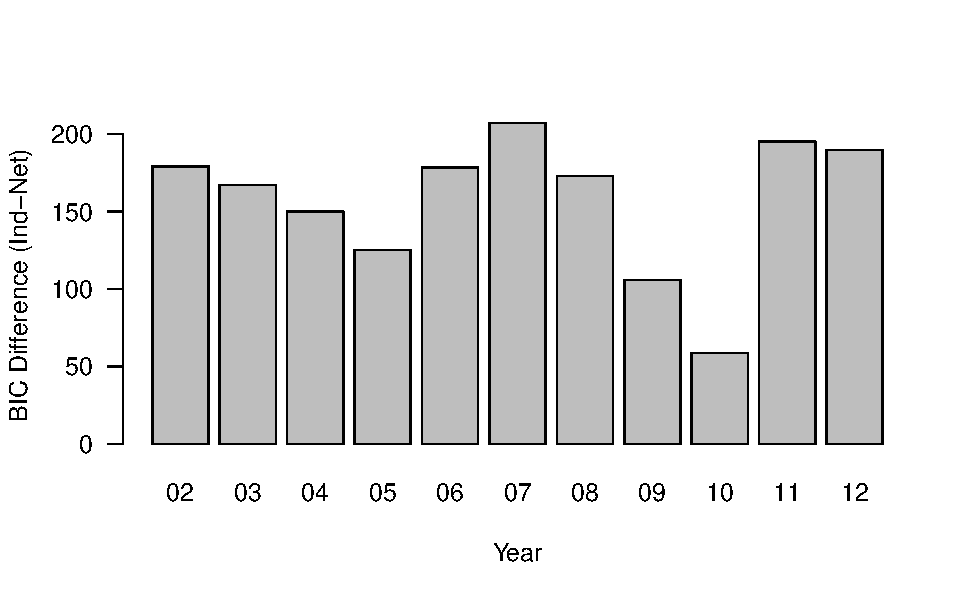
\includegraphics[scale=.75]{draft_figures/BICdiff.pdf} \vspace{-.5cm}
\caption{\label{fig:bic} Difference in BIC between independent and network model.}
\end{figure}


To illustrate how the network model fits better, we compare the fit of the two models to the level of reciprocity in the FDI ties. The level of reciprocity is defined as $$ \frac{ \sum_{(i>j)} \text{\bf 1}\left( \bm{y}_{i,j}>0  \cap \bm{y}_{j,i}>0 \right)}{ \sum_{(i>j)} \text{\bf 1}\left( \bm{y}_{i,j}>0  \cup \bm{y}_{j,i}>0 \right)}.$$ In words, this is the proportion of dyads in which there is an FDI tie from state $i$ to state $j$ and a tie from state $j$ to state $i$ out of the number of dyads in which there is at least one tie. This measures the degree to which the presence of a tie in one direction within a dyad implies that the other tie will exist. To compare the network and independent models we simulated 1,000 networks from each, and compare the reciprocity values in the simulated networks to the observed reciprocity value.
\begin{figure}[!h]
\centering
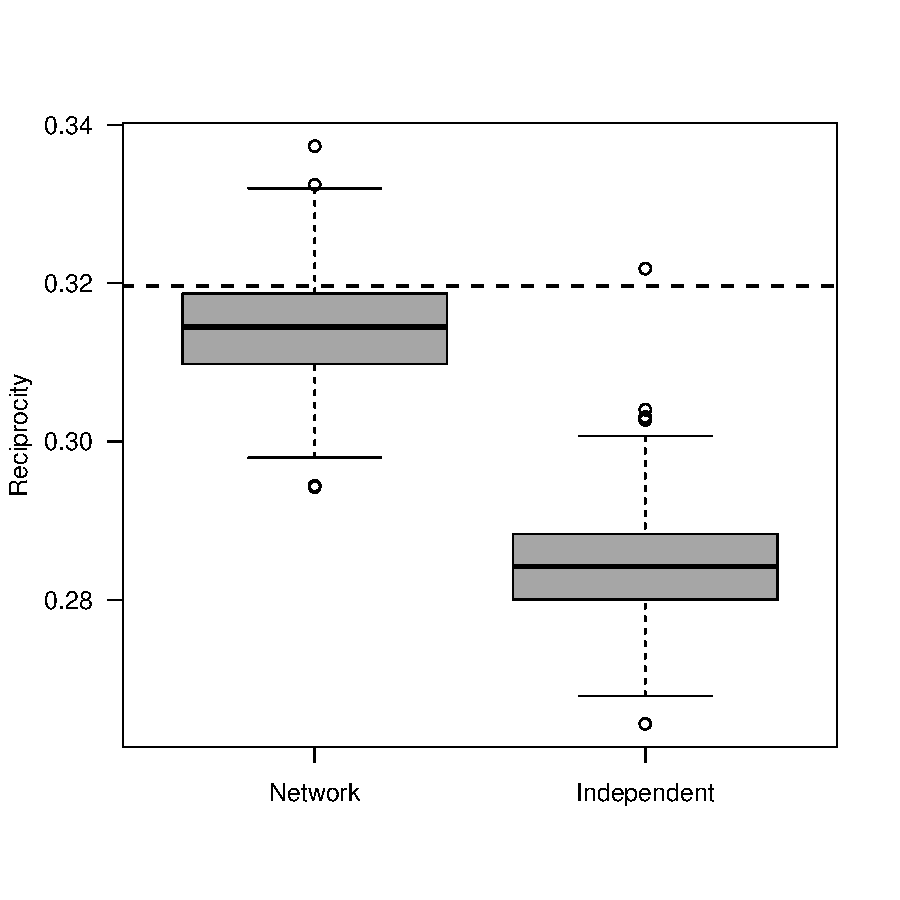
\includegraphics[scale=.75]{draft_figures/reciprocityFit.pdf} \vspace{-.5cm}
\caption{\label{fig:recipFit} Reciprocity values of 1,000 networks simulated from the Network and Independent models. Observed value given by the dashed horizontal line.}
\end{figure}
We see in Figure \ref{fig:recipFit} that the network model provides a much better fit to the observed level of reciprocity (approximately 0.32) than the independent model. Indeed, the observed value is an extreme outlier with respect to the distribution of reciprocity values of networks simulated from the independent model. Unlike the BIC, the fit to the observed reciprocity value does not provide a holistic assessment of model fit. Rather, it illustrates the improved fit to an interpretable quantity in the FDI network, and illustrates how a model in which independence is assumed provides a relatively poor fit to this quantity.







Turning now to the network effects, which are presented in Figure \ref{fig:net_effects}, we see that the reciprocity and transitivity effects are positive and statistically significant in each year, offering robust evidence that FDI flows are interdependent according to these two canonical forms of network structure. \footnote{As noted in the Section 4.1, we also tested our hypotheses on different subsets using different methods of imputation. The majority of these results support our hypotheses, although in the smaller subsets mutuality is not significant for every year estimated. When subsetting based on missingness, we are only left with more developed countries. This indicates that reciprocity might be conditional on the relative level the level of development between dyads.}
\begin{figure}[htp]
\centering
\begin{tabular}{c@{\hskip -.4cm}c}
Reciprocity &
Transitivity\\
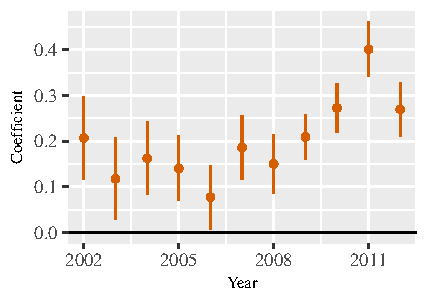
\includegraphics[height=.2\textheight, clip=true, trim=0cm .5cm 0cm .1cm]{draft_figures/rl_plots/Mutuality.pdf}    &
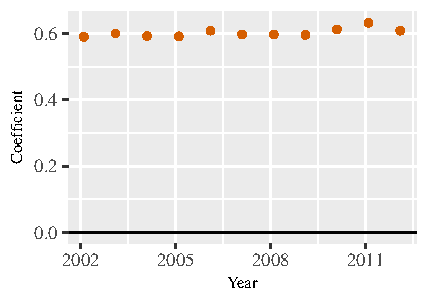
\includegraphics[height=.2\textheight, clip=true, trim=.5cm .5cm 0cm .1cm]{draft_figures/rl_plots/Transitivity.pdf}   \\
\end{tabular}
\caption{\label{fig:net_effects} Estimates of Network terms in Poisson ERGMs. Bars span 95\% confidence intervals.}
\end{figure}
The dependence effects, though formulated intuitively, do not permit a straightforward marginal-effects interpretation of the coefficients aside from the signs of the effects. We can, however, estimate and visualize the dependence effects using simulation. In Figure \ref{fig:interpret} we present visualizations of the effects of the dependence terms. To measure these effects we begin with a simulation exercise in which we simulate networks using both the full model with dependence terms, and the null model based only on covariates. We then classify each simulated edge value in terms of the value of the local version of the dependence term operating on that edge. For example, when it comes to the reciprocity effect, we classify each simulated edge value ($y_{i,j}$) in terms of the value of the mutual edge, $y_{j,i}$. Finally, we estimate the difference in means between the edge values simulated from the full and null models at each dependence term value. This difference in means can be interpreted as the effect on predicted edge values of accounting for the respective dependence term in the model.


We see in Figure \ref{fig:interpret}, that the dependence effects can result in differences in predicted edge values in the range of 1--4 in log-scale FDI.  The standard deviation in log-scale FDI stock (in 2012---the year we use for the interpretation plots) is 2.40.  We see that the scale of both the reciprocity and transitivity effects are significant, with a shift from lower values of the relevant dependence edge to higher values resulting in more than a standard deviation increase in the predicted edge value.
\begin{figure}[!h]
\centering
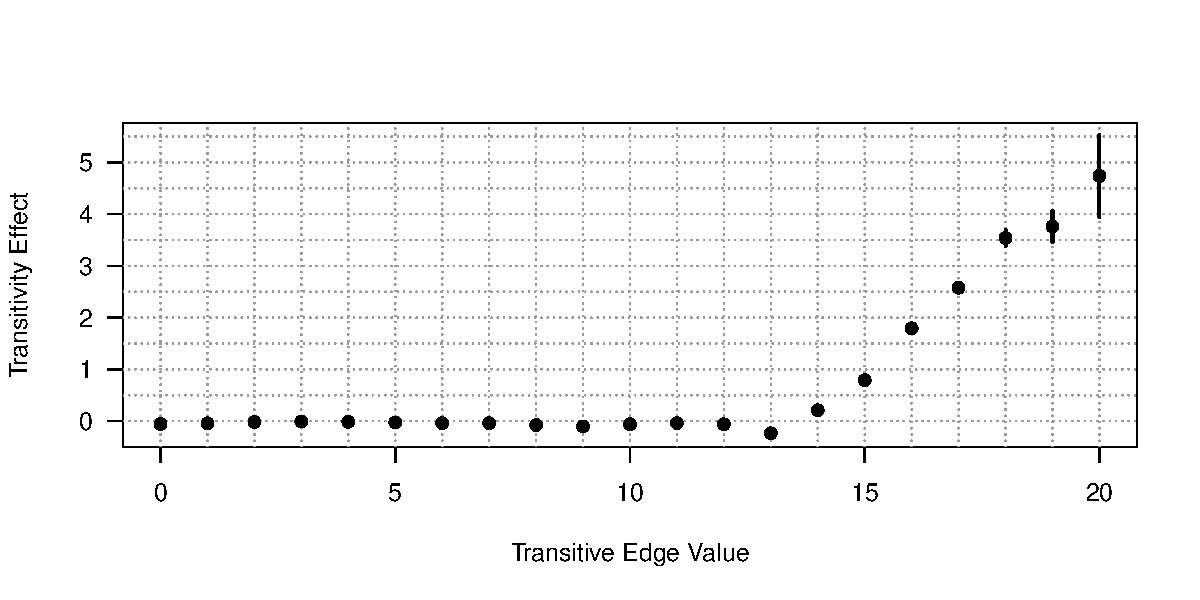
\includegraphics[scale=.75]{draft_figures/transitiveInterpretation.pdf} \vspace{-.5cm}\\
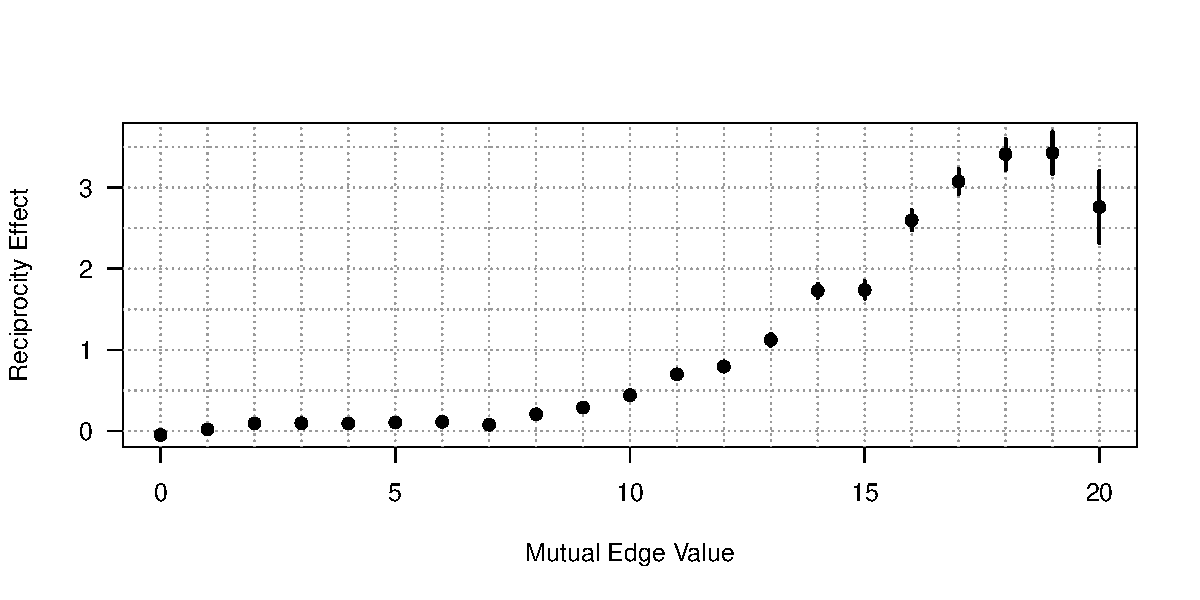
\includegraphics[scale=.75]{draft_figures/mutualInterpretation.pdf} \vspace{-.5cm}
\caption{\label{fig:interpret} Plots depict the difference in predicted value ($y$-axis) that is attributable to the respective dependence effect, averaged over all dyads in the network. Interpretation plots are based on 1,000 FDI stock networks simulated from the 2012 model. Tie weights are measured on the natural logarithm scale. Predicted value differences are calculated by taking the differences between expected dyad values simulated from the full model with dependence terms and the null model that is based on covariates only. Error bars span 95\% confidence intervals for the difference in means. }
\end{figure}

Regarding covariate determinants, presented in Table \ref{fig:effectPlots1}, the results show that FDI flows between a dyad are strongly and positively correlated with the product of the dyad's GDP, BIT, defense treaty, both destination and origin countries' polity scores and trade openness, and origin country's GDP per capita. On the other hand, FDI flows are negatively associated with geographic distance between a dyad, alliance treaty, and destination country's GDP per capita. In addition, we see that the coefficient values are not stable over time. Several parameters such as geographic distance, defense treaty, as well as origin and destination's polity scores, GDP per capita, and trade openness change significantly after 2008 when the Great Recession began. The magnitude of most of these coefficients decreases since then. One possible explanation is that concerns about global economic uncertainty might predominate in investment decisions at that time so that home and host countries' political and economic characteristics play a less important role.


We noted above that omitting dependent network structure, a condition that characterizes previous research on FDI, can result in biased estimates and improper standard errors. For several effects that we include in our models, the results are substantively changed by adding the network parameters. In the network model, we find the following effects to be lower in magnitude, statistically significant in fewer years, or both: Gravity model mass, distance, contiguity, PTA depth, destination polity, destination trade openness, origin trade openness, origin GDP per capita, origin polity, and origin trade openness. For each of these effects, our results indicate that omitting the network dependencies lead to either an overestimate of the effect of the respective variable, or worse, a Type 2 inferential error in which the null hypothesis of no effect is incorrectly rejected. This finding shows that, even if a researcher is not theoretically interested in network dependencies, (s)he should still incorporate them into an empirical model in order to avoid misspecification bias.

For the Poisson-reference ERGM these covariate estimates are interpreted by exponentiating Euler's constant to the power of the coefficient times the number of unit changes in the covariate to get the expected change in the tie weight. We've simplified this as all covariates were normalized to be between zero and one. Therefore, a one unit change in the covariate is a change from the minimum value to the maximum value in the observed covariate values. Taking Polity, in-degree for example, if the FDI destination had a Polity score of 10 in 2002, we would expect the value of logged FDI being sent to be 1.011 times more than a destination that had a Polity score of -10. In the model with network terms this expected increase is only 1.008 times higher. 

\pagebreak
\begin{longtable}{c@{\hskip -.4cm}c}
Sum of Edges&
Sum Sqrt. of Edges\\
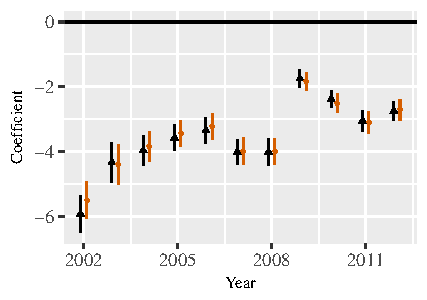
\includegraphics[height=.2\textheight, clip=true, trim=0cm .5cm 0cm .1cm]{draft_figures/rl_plots/Sum.pdf}    &
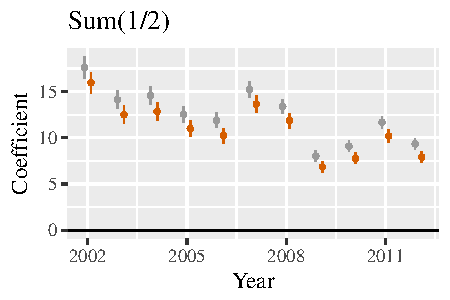
\includegraphics[height=.2\textheight, clip=true, trim=.5cm .5cm 0cm .1cm]{draft_figures/rl_plots/Sum_5.pdf}   \\
Number of Non-Zero Edges &
Lagged FDI Flow\\
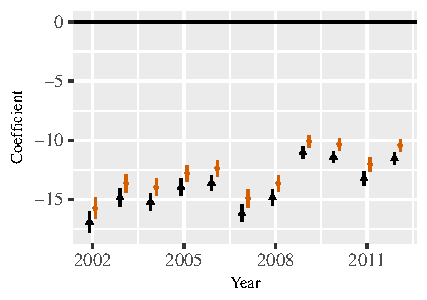
\includegraphics[height=.2\textheight, clip=true, trim=0cm .5cm 0cm .1cm]{draft_figures/rl_plots/Nonzero.pdf} &
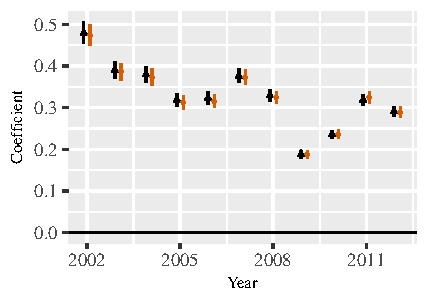
\includegraphics[height=.2\textheight, clip=true, trim=.5cm .5cm 0cm .1cm]{draft_figures/rl_plots/LDV.pdf}   \\
Log-GDP Product &
Log-Geographic Distance\\
\includegraphics[height=.2\textheight, clip=true, trim=0cm .5cm 0cm .1cm]{draft_figures/rl_plots/GDP_Dyad.pdf}    &
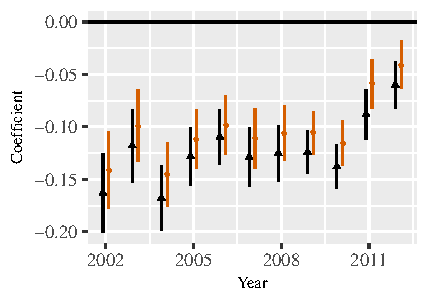
\includegraphics[height=.2\textheight, clip=true, trim=.5cm .5cm 0cm .1cm]{draft_figures/rl_plots/Distance.pdf}   \\
\pagebreak
Defense Treaty &
Alliance Treaty\\
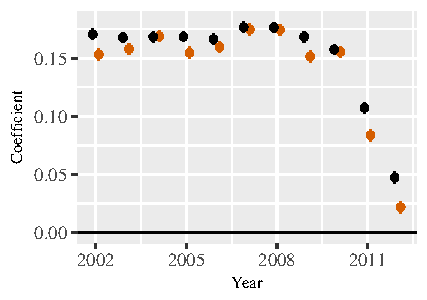
\includegraphics[height=.2\textheight, clip=true, trim=0cm .5cm 0cm .1cm]{draft_figures/rl_plots/Defense.pdf}   &
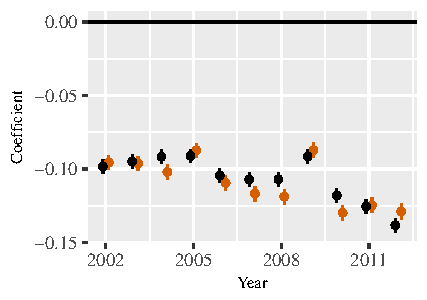
\includegraphics[height=.2\textheight, clip=true, trim=.5cm .5cm 0cm .1cm]{draft_figures/rl_plots/Alliance.pdf}\\

%
%\pagebreak
%

Polity, in-degree &
Polity, out-degree\\
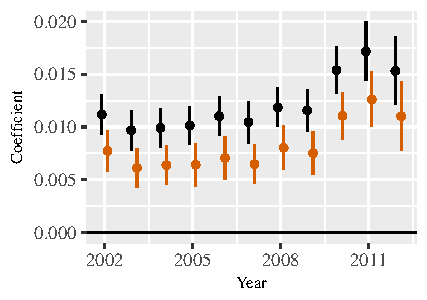
\includegraphics[height=.2\textheight, clip=true, trim=0cm .5cm 0cm .1cm]{draft_figures/rl_plots/Polity_in.pdf}   &
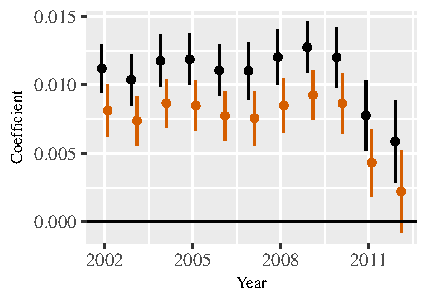
\includegraphics[height=.2\textheight, clip=true, trim=.5cm .5cm 0cm .1cm]{draft_figures/rl_plots/Polity_out.pdf}   \\
GDP per capita, in-degree &
GDP per capita,  out-degree\\
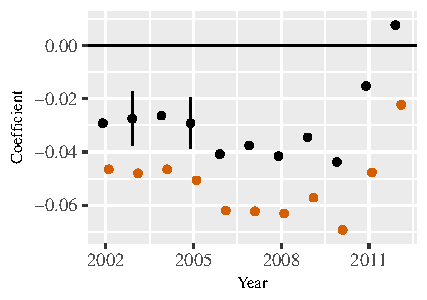
\includegraphics[height=.2\textheight, clip=true, trim=0cm .5cm 0cm .1cm]{draft_figures/rl_plots/GDPpc_in.pdf} &
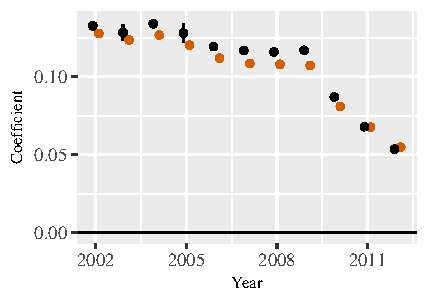
\includegraphics[height=.2\textheight, clip=true, trim=.5cm .5cm 0cm .1cm]{draft_figures/rl_plots/GDPpc_out.pdf}   \\
Bilateral Investment Treaty &
Bilateral Trade Volume\\
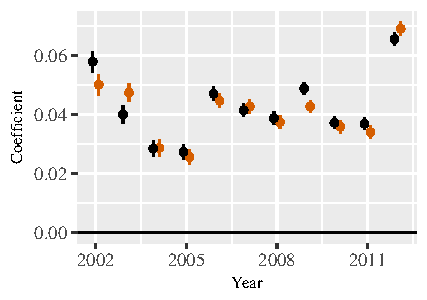
\includegraphics[height=.2\textheight, clip=true, trim=0cm .5cm 0cm .1cm]{draft_figures/rl_plots/BIT.pdf}    &
\includegraphics[height=.2\textheight, clip=true, trim=.5cm .5cm 0cm .1cm]{draft_figures/rl_plots/TradeV.pdf}   \\
Trade Openness, in-degree &
Trade Openness,  out-degree\\
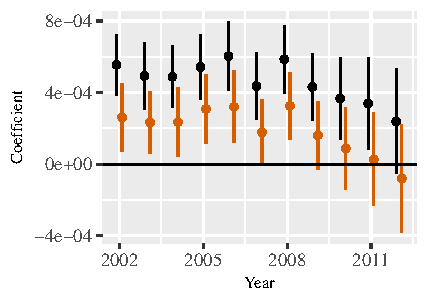
\includegraphics[height=.2\textheight, clip=true, trim=0cm .5cm 0cm .1cm]{draft_figures/rl_plots/TradeO_in.pdf}  &
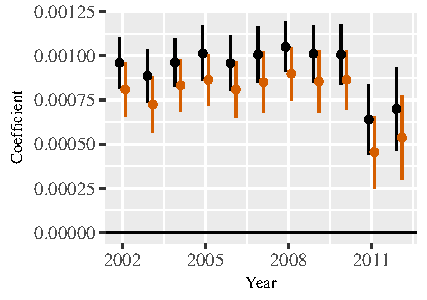
\includegraphics[height=.2\textheight, clip=true, trim=.5cm .5cm 0cm .1cm]{draft_figures/rl_plots/TradeO_out.pdf}   \\

\caption{\label{fig:effectPlots1} Estimates of exogenous terms in Poisson ERGMs. Bars span 95\% confidence intervals. Black coefficient representations are from models excluding dependence terms (i.e., transitivity and reciprocity).}

\end{longtable}

\subsection{Ripple effects of FDI shocks}\label{contagion}

When it comes to the analysis of the international political economy, one of the central advantages of the network scientific perspective is that it sheds light on the interdependence in the system. As we reviewed above, economic contagion has been largely theorized as the ways in which country-level economic conditions can spread through the edges in an economic network. Our analysis reflects a different form of interdependence---characterizing the ways in which the edges in the network depend upon each other. The ERGM provides a framework for investigating the patterns of dependence among edges in order to understand how edges in the network depend upon each other. In this section we present an analysis of how a simple shock to the FDI network---the elimination of a single edge---affects the expected values of the edges that are ``close'' to the eliminated edge. The complete elimination of a single FDI edge would be admittedly rare, but the effects would be similar to that of a large reduction in an edge value and simulating the network conditional on a fixed but non-zero edge value is much more computationally complex than eliminating an edge entirely. Another way to look at edge elimination is to consider the structural differences we would have observed if a policy was in place to prevent investment along a particular edge (e.g., via an embargo on investment). This exercise contributes to our understanding of contagion and domino effects in the international economic system.

We investigate the interdependence in the FDI network by simulating networks from the full model estimated for 2012. Our conclusions are robust to using other years---we use 2012 for consistency with the model interpretations presented above. Our objective in this simulation experiment is to understand how the elimination of an FDI edge from country $i$ to country $j$ affects the other ties to which countries $i$ and $j$ are incident. Specifically, we analyze the effects of eliminating edge $i \rightarrow j$  on four measures: (1) the expected value of FDI ties sent by $i$ to countries other than $j$, (2) the expected value of FDI ties sent by $j$, (3) the expected value of ties received by $i$, and (4) the expected value of ties received by $j$ from countries other than $i$.  These edges are ``close'' to edge $i \rightarrow j$ according to our ERGM specification in that (1) the edge sent from $j$ to $i$ factors directly into the measure of reciprocity, and (2) all edges sent to (from) $i$ and $j$ by other nodes factor into the transitive triads measure with the edge from $i$ to $j$.

There are three steps in the simulation experiment we conduct to analyze the effects of eliminating edge $i \rightarrow j$. We first simulate 500 networks from the 2012 ERGM fit. We use this sample to calculate expected values of each edge, as well as our summary measures of indirect effects, from the model without constraints on edge values (i.e., no edges eliminated). Our second step is to, for each observed edge in the 2012 networks, simulate 100 networks from the ERGM with the same parameter values, but with the respective edge value fixed to zero. Our third step is to calculate, again for each edge, the percentage change in the measures of indirect effects that result from eliminating the edge.

\begin{figure}[!h]
\centering
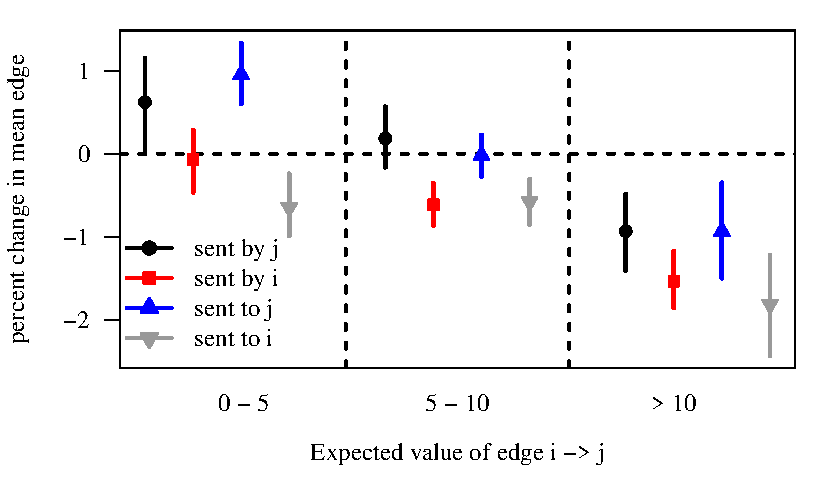
\includegraphics[scale=.85]{./draft_figures/contagion_simulation_results} \vspace{-.5cm}\\
\caption{\label{fig:contagion} Results from simulation exercise investigating the effects of eliminating edge $i \rightarrow j$ on the expected values of other edges incident to both $i$ and $j$. Points are drawn at the average values over all edges in the 2012 network. The bars span 95\% nonparametric bootstrap confidence intervals, which are constructed by resampling edges.  Expected values of edges are expressed on the natural logarithm scale.}
\end{figure}

The results from our simulation exercise are presented in Figure \ref{fig:contagion}. We divide the edges in the network into three categories based on their expected values---small edge values (approximately 40\% of edges), between 0 and 5 on the log scale (i.e., \$150m USD or less); medium edge values (approximately 50\% of edges), between 5 and 10 on the log scale (\$150m- \$22bn USD); large edge values (approximately 10\% of edges), greater than 10 on the log scale (\$22bn USD and above). We see that the effects of eliminating small and medium sized edges are mixed. The adverse effects are confined to the sending country $i$ itself. This result could be attributable to the inability to detect domino effects of a relatively small perturbation to the network---the elimination of a single edge---when the edge's value is small. However, as the expected value of the edge being eliminated increases, a consistent signal emerges. For large edges, eliminating edge $i \rightarrow j$ from the network reduces the expected values of other edges sent to/from nodes $i$ and $j$ by 1-2\%. When multiplied over dozens, or even hundreds, of ties to which two countries are incident, a 1-2\% decrease in the value of investments would represent a substantial economic shock. For example, a economic crisis in countries at the center of the network, such as the U.S., will have a ripple effect on FDI inflows and outflows in many other countries with which the U.S. even doesn't have a direct investment tie. Therefore, the cost of any disruption to the network is multiplied by the interdependence. This simulation exercise illustrates the consequences of interdependence in FDI networks.









\section{Conclusion}
% paragraph on substantive finding

Over recent decades, one prominent feature of the global economy is the growth of global production networks. Firms have chosen to invest overseas at an unprecedented level, and consequently, production is increasingly fragmented and organized across the globe. One central question is then what accounts for the pattern of global investment flows. In this paper, we adopt a novel network approach to address this question. FDI flows represent ties between states that arise through both a complex underlying network of inter and intra-firm relations, and legal agreements between states. The relational backdrop through which FDI operates leads to predictable network structure in the patterns of ties formed through FDI. We present a network theory of FDI that includes reciprocity and transitivity as the core structural dependencies. The results of our statistical models confirm that these dependencies exist---a result that holds over time, and while adjusting for other covariates known to relate to FDI.

%Our result bears important real-world implications, as network dependencies will lead the effects of policies relevant to FDI to ripple through the network according to these dependencies. In FDI networks, a country's ability to attract foreign investment depends not only on its own locational advantages such as factor endowments, large consumer markets, or favorable government policies, but also on its connectivity to existing partner states in the network. As such, network dependencies will demand more policy coordination among nations, and thus, more likely to promote cooperation and peace \citep[see,~e.g.,][]{Kim_Solingen:2017,Dorussen_Ward:2008,Dorussen_Ward:2010}.


We should emphasize that our theory, specification, and finding of network-wide reciprocity and transitivity represent just the start in a broader scholarly dialogue on the network science of FDI flows. One limitation of our study is that we do not model any forms of conditional variation in reciprocity and transitivity. In theory, we should expect that the degree of reciprocity varies by countries' levels of development. Investing abroad incurs large fixed costs and firms need to overcome the disadvantages such as liability of foreignness they face when competing with indigenous firms in the host country. Therefore, only the most productive firms are able to engage in FDI activities \citep{Melitz:2003,Helpman_et_al:2004}. Historically, MNCs from developed countries predominate. Although there is a surge of FDI from developing countries since the early 2000s, firms in most developing countries are still not competitive enough to strive in a global market.\footnote{For instance, in 2005 outward FDI flows and stocks from developing countries are approximately 17\% and 13\% of the world total, respectively \citep{UNCTAD:2006}. Furthermore, outward FDI from developing countries is highly concentrated; the top 10 countries, mostly large emerging economies such as Argentina, Brazil, Chile, China, Mexico, Russia, and South Africa contribute about 83\% \citep{UNCTAD:2006}. } It is important to explore how network dependencies vary across different groups of countries.

Future research could look into the political and economic consequences of FDI networks. In this article, we take a first step to model the characteristics of FDI networks and show that they exhibit both reciprocity and transitivity. The methodological advancement now allows researchers to examine the effects of the global structure of the network on states. Given the dramatic expansion of global production networks and states are increasingly tied to each other through multinationals' investment activities, it is pivotal to understand the consequences of FDI networks, such as how the networks transmit exogenous shocks, influence domestic politics, and shape international cooperation and conflict.




\newpage
\singlespacing
\bibliographystyle{apsr}
\bibliography{fdi_reference}


\newpage
\doublespacing
\setcounter{page}{1}
\setcounter{figure}{0}
\setcounter{footnote}{0}
\setcounter{equation}{0}
\setcounter{table}{0}
\renewcommand{\thesection}{Appendix \Alph{section}}
\renewcommand\thetable{\Alph{table}}
\renewcommand\thefigure{\Alph{figure}}
\appendix
\section{Summary Statistics}\label{summstats}

\begin{longtable}{c@{\hskip -.4cm}c}
Alliance Treaty &
Defense Treaty\\
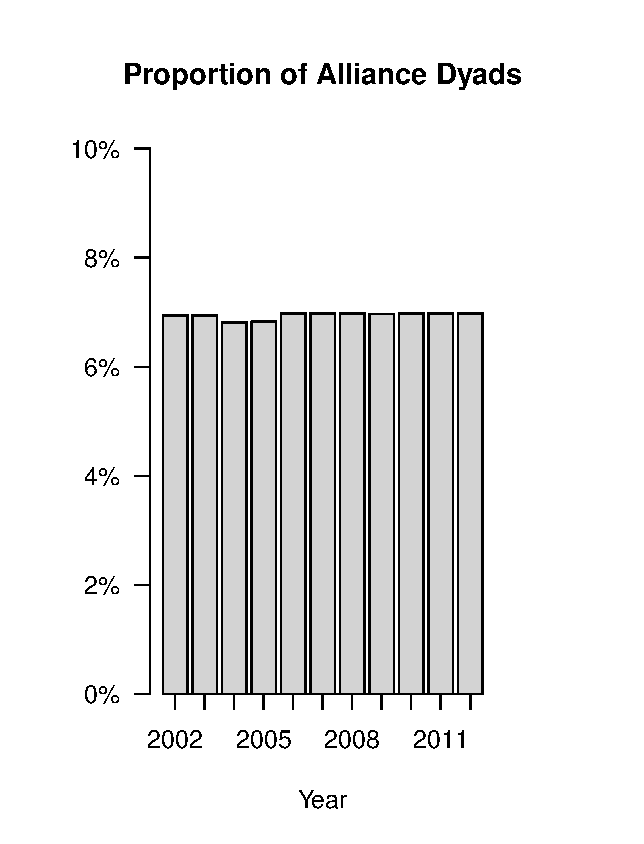
\includegraphics[height=.2\textheight, clip=true, trim=0cm 1cm 0cm 1.6cm]{draft_figures/descriptive_plots/alliance.pdf}    &
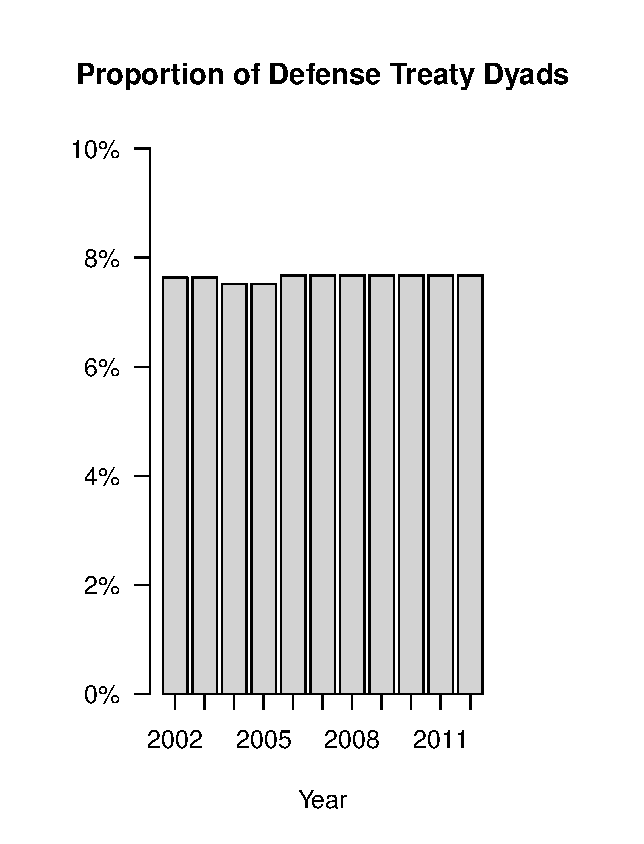
\includegraphics[height=.2\textheight, clip=true, trim=.5cm 1cm 0cm 1.6cm]{draft_figures/descriptive_plots/defense.pdf}   \\
Bilateral Investment Treaty &
Polity\\
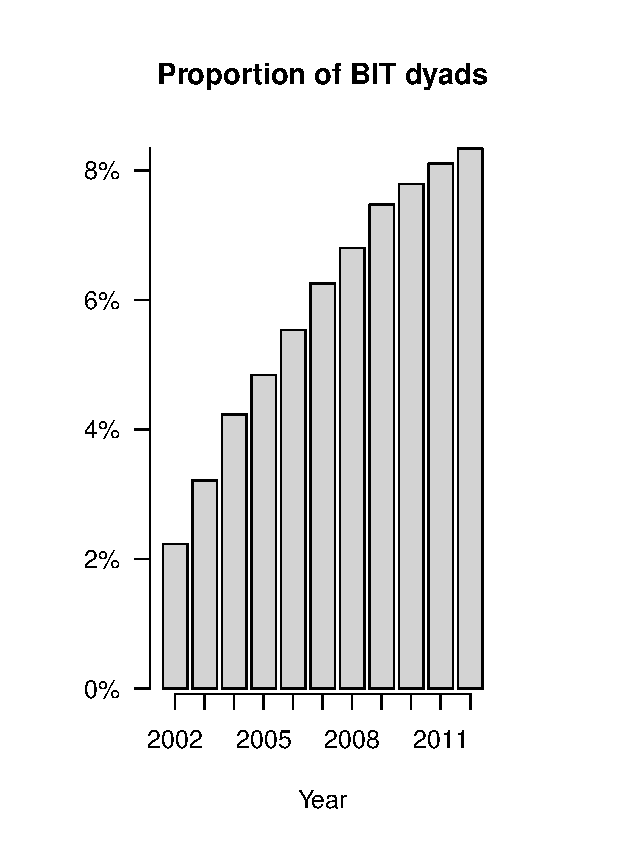
\includegraphics[height=.2\textheight, clip=true, trim=0cm 1cm 0cm 1.6cm]{draft_figures/descriptive_plots/BIT.pdf}    &
\includegraphics[height=.2\textheight, clip=true, trim =1cm 1cm 0cm 1.6cm]{draft_figures/descriptive_plots/Polity.pdf}   \\
Dyad GDP Product &
Distance\\
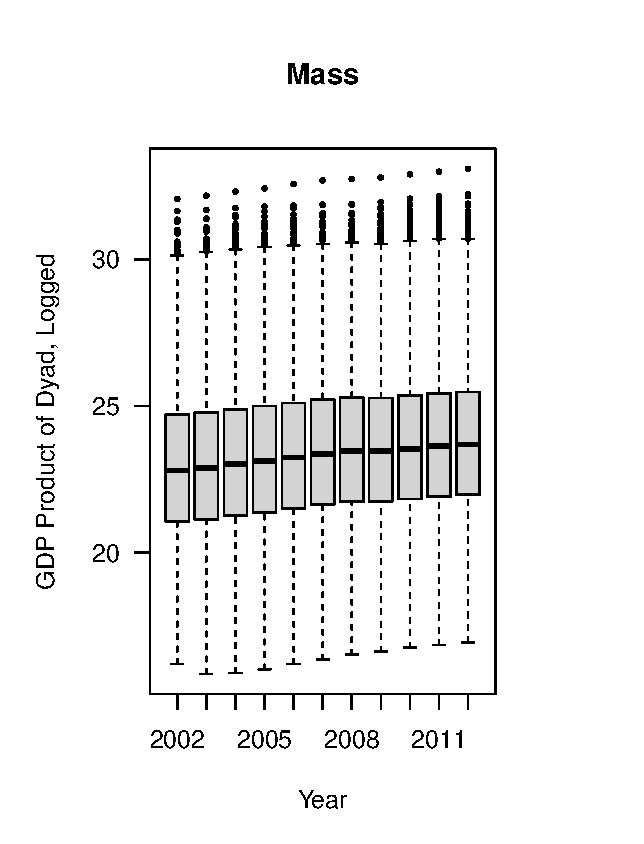
\includegraphics[height=.2\textheight, clip=true, trim=1cm 1cm 0cm 1.6cm]{draft_figures/descriptive_plots/mass.pdf}    &
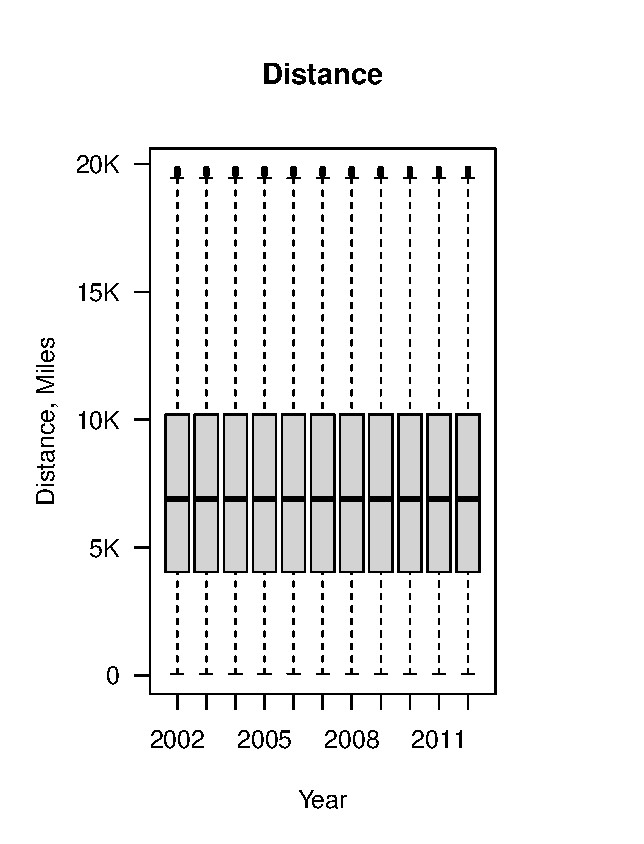
\includegraphics[height=.2\textheight, clip=true, trim=1cm 1cm 0cm 1.6cm]{draft_figures/descriptive_plots/distance.pdf}   \\

\pagebreak

GDP per capita &
Trade as \% of GDP\\
\includegraphics[height=.2\textheight, clip=true, trim=1cm 1cm 0cm 1.6cm]{draft_figures/descriptive_plots/GDPpc.pdf}    &
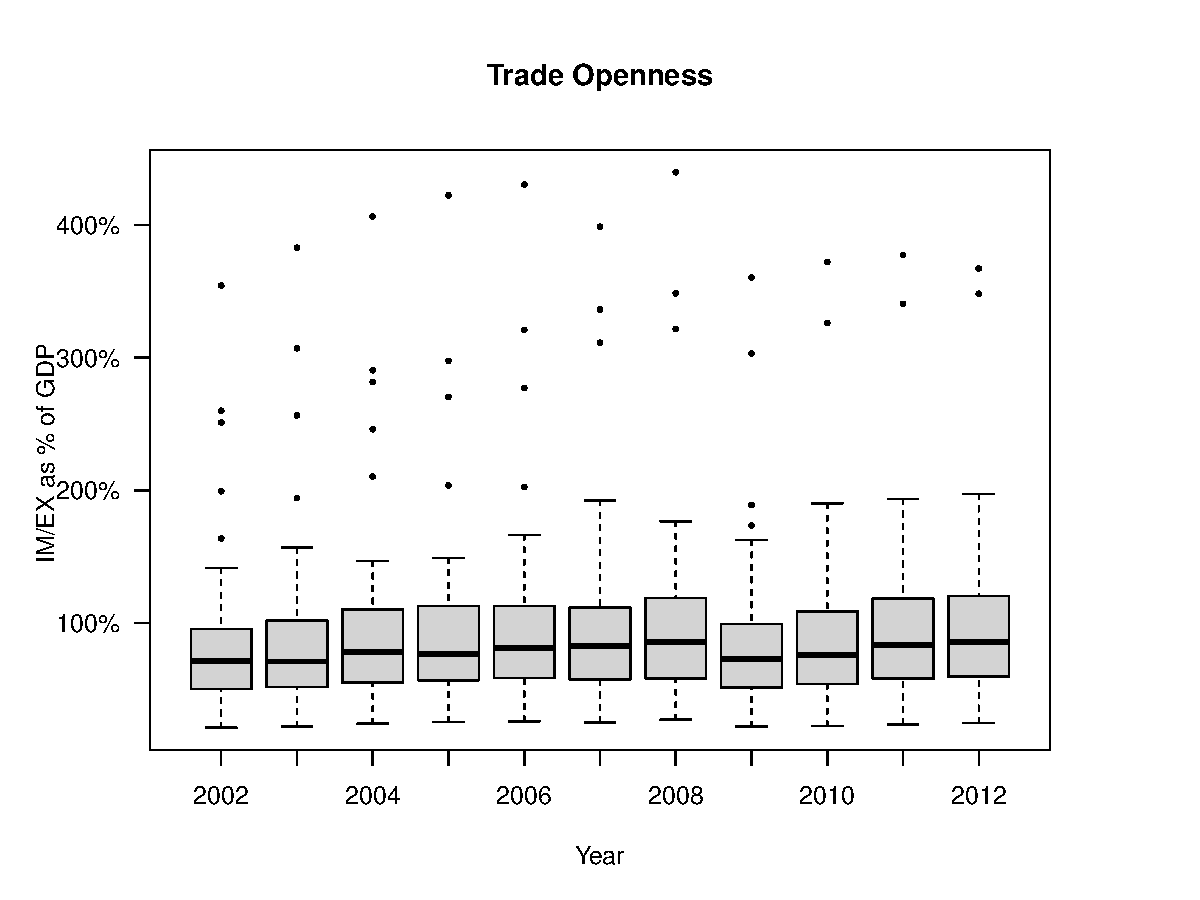
\includegraphics[height=.2\textheight, clip=true, trim=.95cm 1cm 0cm 1.6cm]{draft_figures/descriptive_plots/TradeO.pdf}   \\
Trade Volume &
FDI Stock\\
\includegraphics[height=.2\textheight, clip=true, trim=1cm 1cm 0cm 1.6cm]{draft_figures/descriptive_plots/TradeV.pdf}    &
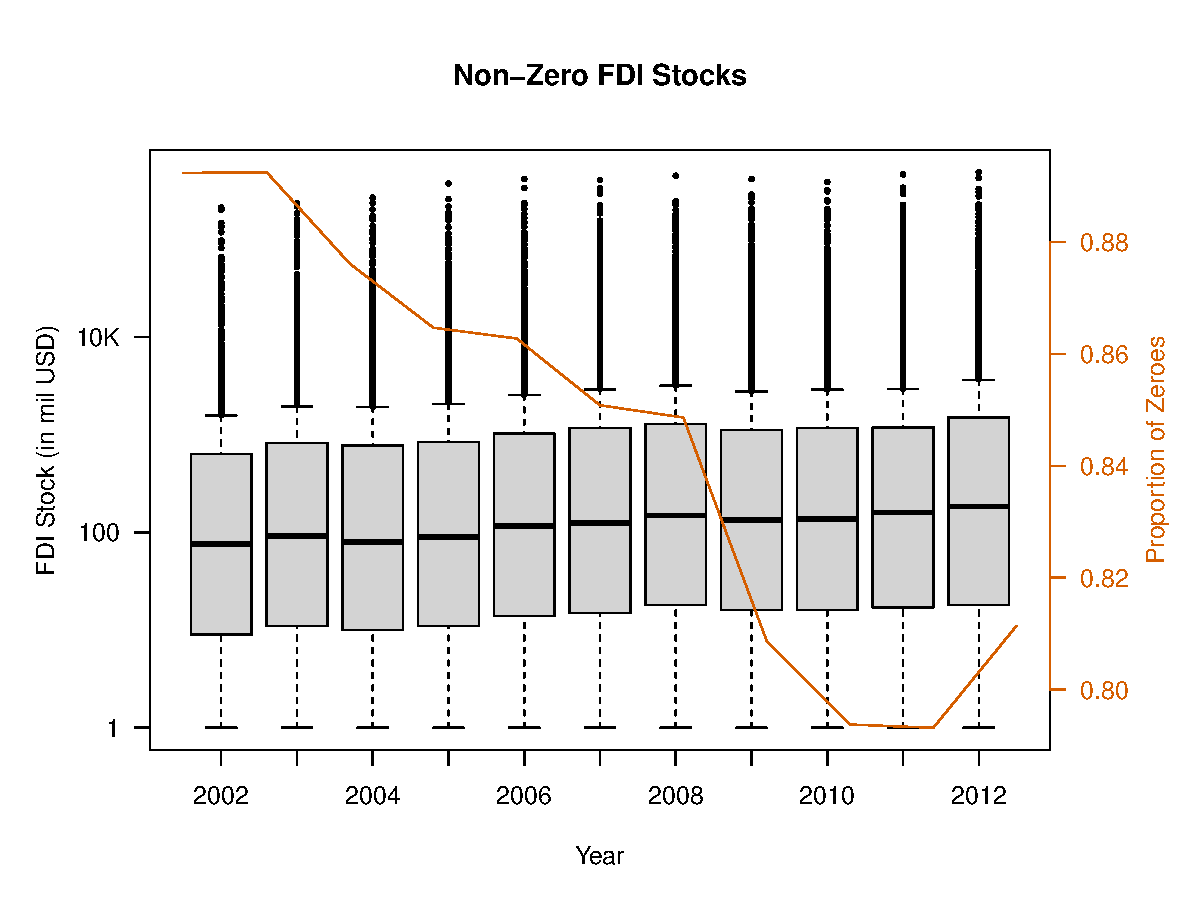
\includegraphics[height=.2\textheight, clip=true, trim=1cm 1cm 0cm 1.6cm]{draft_figures/descriptive_plots/fdi_stock.pdf}   \\

\caption{\label{fig:sum_stats} Summary Statistics.}
\end{longtable}


\clearpage
\begin{table}[!htbp] \centering
  \caption{Correlation Matrix}
  \label{}
\begin{tabular}{@{\extracolsep{5pt}} lccccccccc}
\\[-1.8ex]\hline
\hline \\[-1.8ex]
 & Mass & Distance & Polity \\
\hline \\[-1.8ex]
Mass & $1$ & $$-$0.003$ & $0.091$   \\
Distance (logged) & $$-$0.003$ & $1$ & $0.008$  \\
Polity & $0.091$ & $0.008$ & $1$  \\
Trade Openness & $$-$0.166$ & $$-$0.057$ & $$-$0.078$ \\
BITs & $0.141$ & $$-$0.085$ & $0.018$  \\
Trade Volume & $0.714$ & $$-$0.215$ & $0.215$   \\
GDP per capita (logged)& $0.392$ & $$-$0.084$ & $0.166$   \\
Alliance Treaty & $0.133$ & $$-$0.348$ & $0.073$   \\
Defense Treaty & $0.065$ & $$-$0.391$ & $0.065$ \\
\hline \\[-1.8ex]
\\[-1.8ex]\hline
\hline \\[-1.8ex]
 & Trade Openness &BITs &  Trade Volume  \\
\hline \\[-1.8ex]
Mass & $$-$0.166$ & $0.141$& $0.714$  \\
Distance (logged) & $$-$0.057$ & $$-$0.085$ & $$-$0.215$ \\
Polity & $$-$0.078$ & $0.018$& $0.215$  \\
Trade Openness  & $1$ & $0.032$ & $$-$0.055$ \\
BITs & $0.032$ & $1$ & $0.143$ \\
Trade Volume & $$-$0.055$ & $0.143$& $1$  \\
GDP per capita (logged) & $0.225$ & $0.093$ & $0.330$  \\
Alliance Treaty & $$-$0.044$ & $0.021$& $0.216$  \\
Defense Treaty & $$-$0.046$ & $0.010$ & $0.177$   \\
\hline \\[-1.8ex]
\\[-1.8ex]\hline
\hline \\[-1.8ex]
& GDP per capita & Alliance Treaty & Defense Treaty \\
\hline \\[-1.8ex]
Mass & $0.392$ & $0.133$ & $0.065$ \\
Distance & $$-$0.084$ & $$-$0.348$ & $$-$0.391$  \\
Polity & $0.166$ & $0.073$ & $0.065$   \\
Trade Openness & $0.225$ & $$-$0.044$ & $$-$0.046$\\\
BITs & $0.093$ & $0.021$ & $0.010$\\
Trade Volume & $0.330$ & $0.216$ & $0.177$ \\
GDP per capita (logged) & $1$ & $0.098$ & $0.038$ \\
Alliance Treaty & $0.098$ & $1$ & $0.850$ \\
Defense Treaty & $0.038$ & $0.850$ & $1$ \\
\hline \\[-1.8ex]
\end{tabular}
\end{table}

\begin{figure}[!h]
\centering
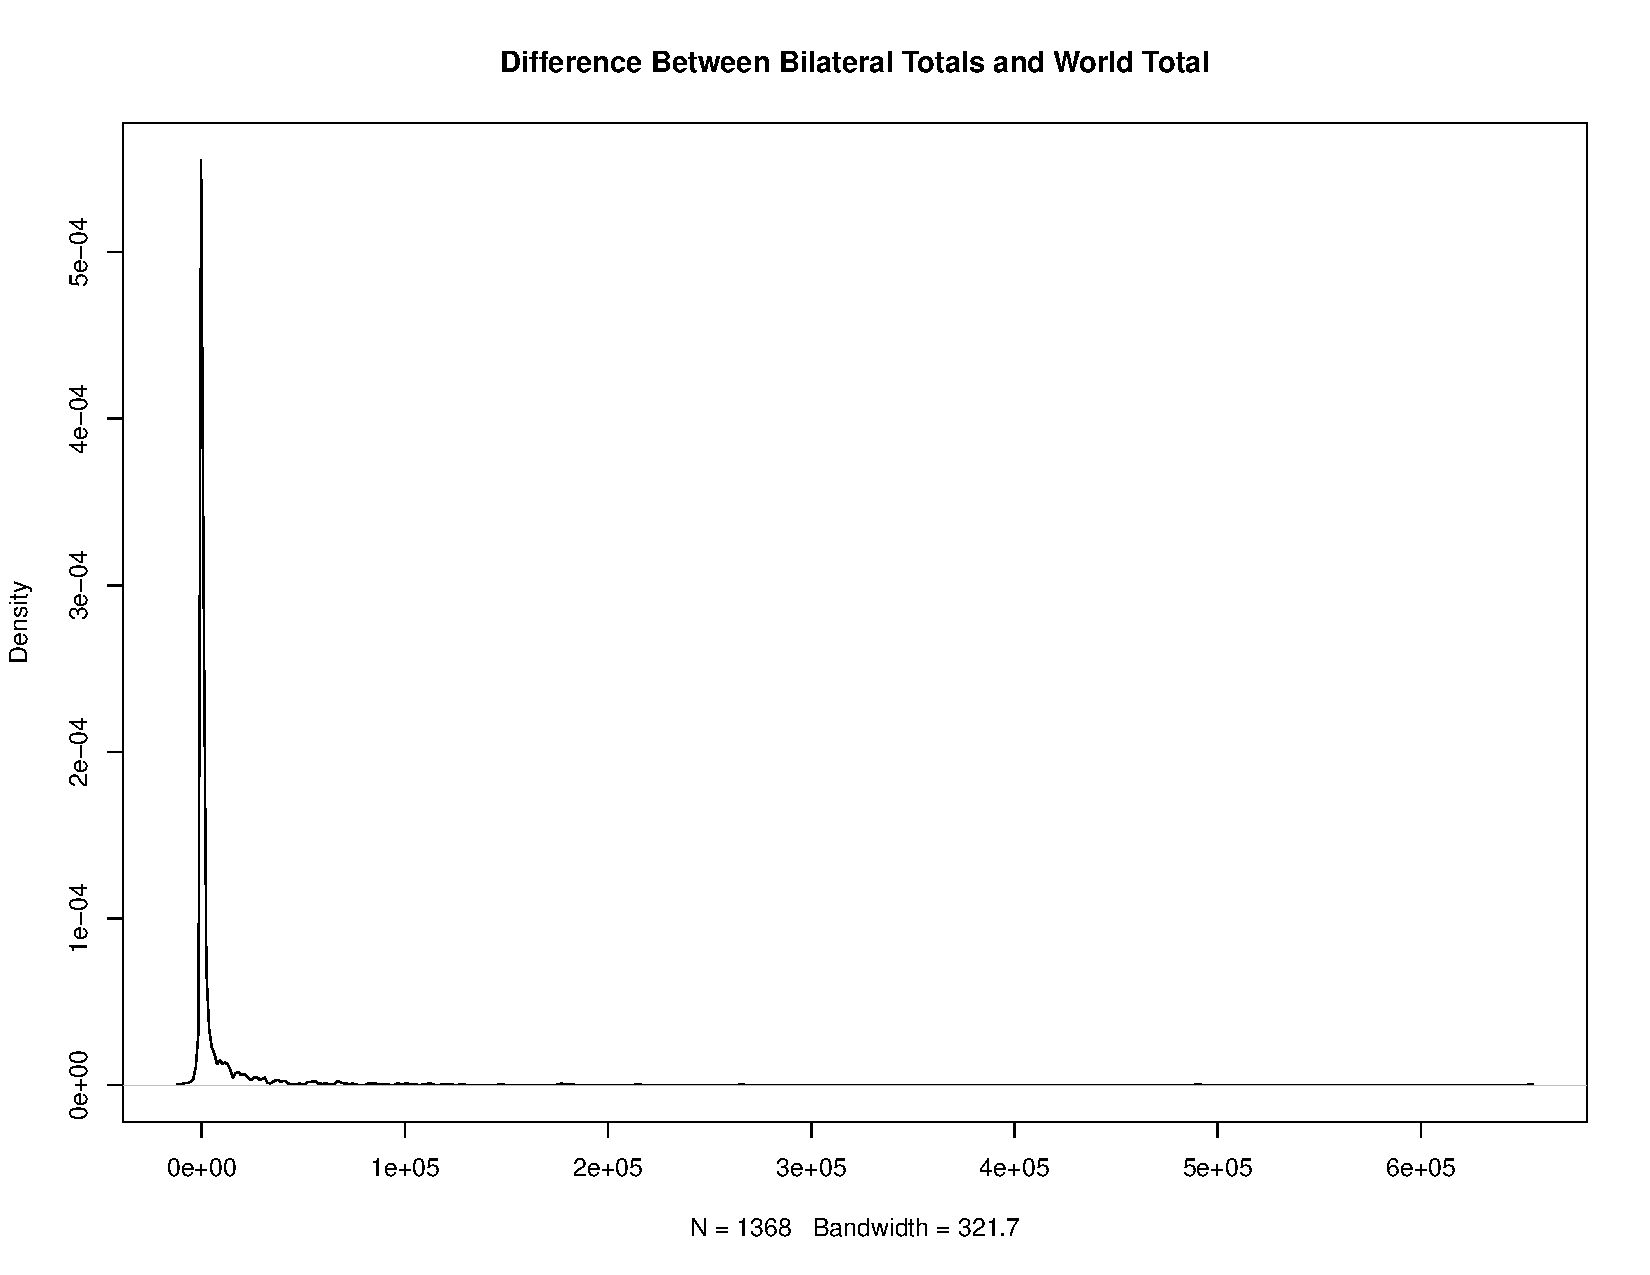
\includegraphics[height=5in]{draft_figures/descriptive_plots/diff_plot.pdf} \vspace{0cm}
\caption{\label{fig:flows} Density Plot of the Difference between Total FDI stocks and Summing Bilateral FDI stocks.}
\end{figure}



%\clearpage
%\begin{figure}[!h]
%\centering
%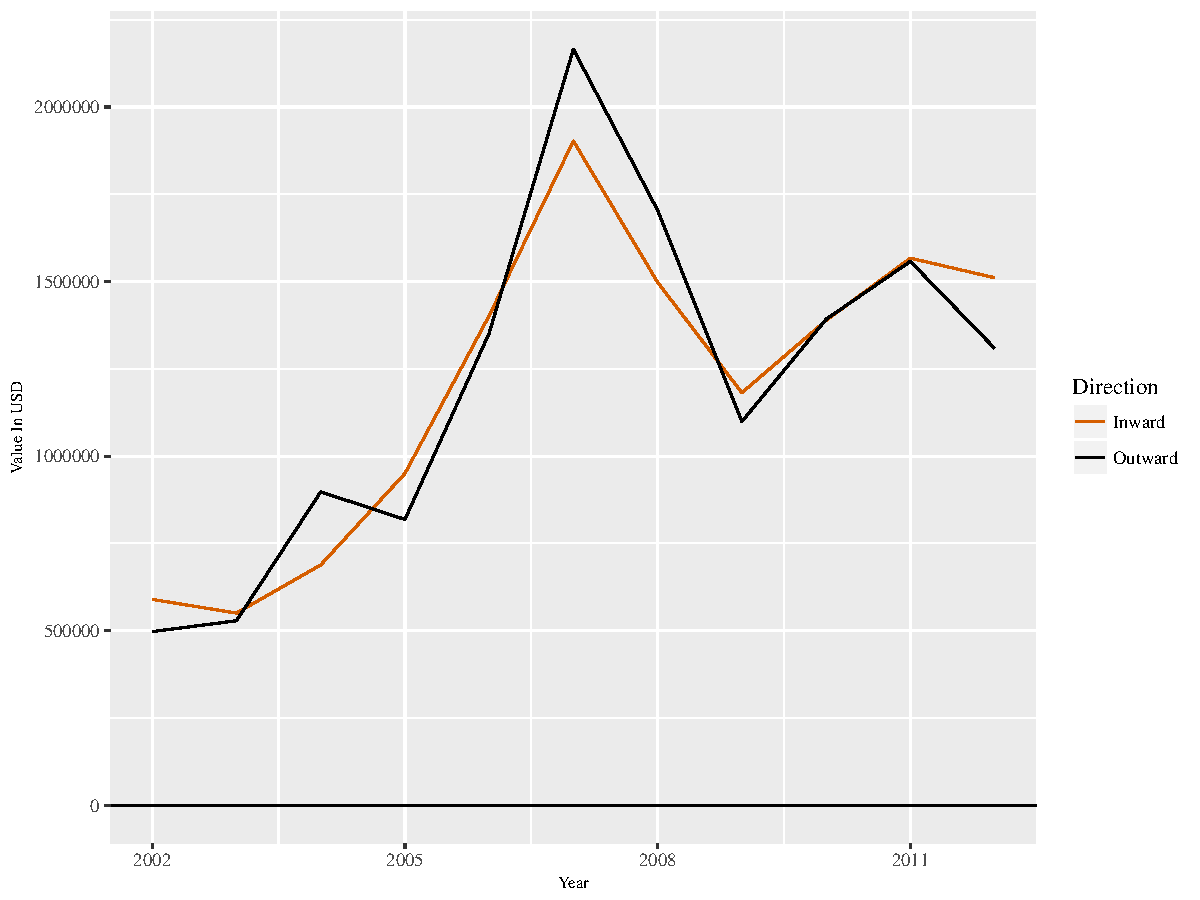
\includegraphics[height=3.5in]{draft_figures/descriptive_plots/fdi_flows.pdf} \vspace{0cm}
%\caption{\label{fig:flows} Global FDI flows by Direction.}
%\end{figure}


\clearpage

\section{Time-Pooled Model Results}\label{pooledresults}
For robustness checks, we re-estimate the count ERGM by pooling the data, which is common in the literature for regression based models. Figure \ref{fig:exog_2} shows that after pooling, network terms remain positive and statistically significant, supporting our hypothesis that reciprocity and transitivity characterize FDI flows. The exogenous covariates from the pooled model are presented in Table \ref{fig:effectPlots2}. The estimates are similar to yearly results in terms of direction and statistical significance. %As expected from pooling, there are decreases in standard errors because the increased number of observations. %for variables that exhibit more yearly heterogeneity, estimates are on average more different than yearly estimates.

\begin{figure}[!h]
\centering
\begin{tabular}{c@{\hskip 0cm}c}
Reciprocity & Transitivity \\
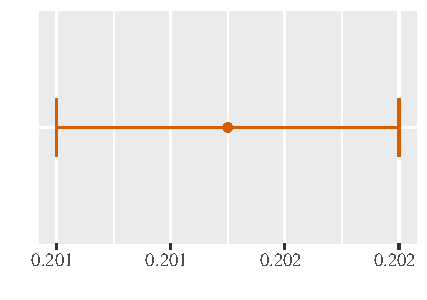
\includegraphics[height=.2\textheight, clip=true, trim=0cm 0cm 0cm .2cm]{draft_figures/plots_pooled/Mutuality.pdf}    &
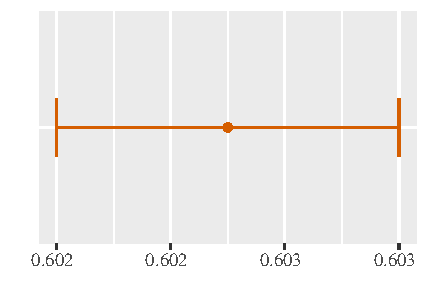
\includegraphics[height=.2\textheight, clip=true, trim=0cm 0cm 0cm .2cm]{draft_figures/plots_pooled/Transitivity.pdf}
\end{tabular}
\caption{\label{fig:exog_2} Estimates of Dependence terms in time-pooled ERGMs. Bars span 95\% confidence intervals. }
\end{figure}


The results also show that ignoring network structure lead to biased estimates in several covariates. We see significant differences in the coefficients for distance, the product of dyad's GDP, the three treaty variables, as well as origin and destination's GDP per capita, Polity, and trade openness. These findings are consistent with those from the yearly models. It illustrates that failure to include network structure results in biased estimates.

\clearpage
\begin{longtable}[!h]{c@{\hskip 0cm}c}
Sum & Sum$^{(1/2)}$ \\
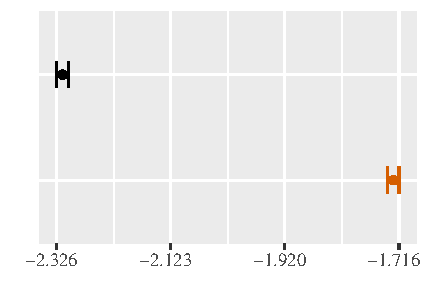
\includegraphics[height=.18\textheight, clip=true, trim=0cm 0cm 0cm .2cm]{draft_figures/plots_pooled/Sum.pdf}    &
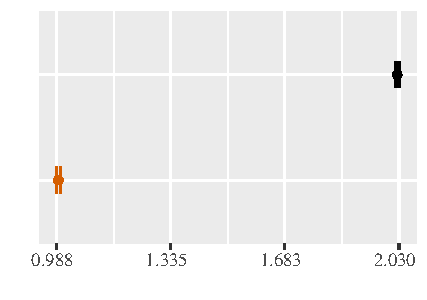
\includegraphics[height=.18\textheight, clip=true, trim=0cm 0cm 0cm .2cm]{draft_figures/plots_pooled/sum_5.pdf}   \\
%\pagebreak
Non-Zero & Alliance Treaty\\
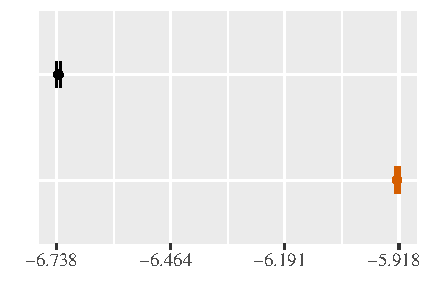
\includegraphics[height=.18\textheight, clip=true, trim=0cm 0cm 0cm .2cm]{draft_figures/plots_pooled/Non-zero.pdf} &
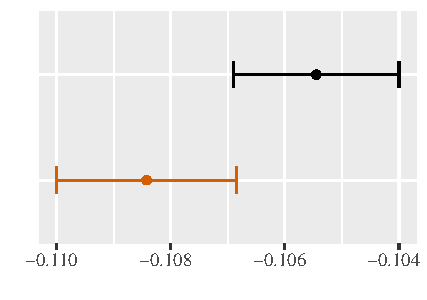
\includegraphics[height=.18\textheight, clip=true, trim=0cm 0cm 0cm .2cm]{draft_figures/plots_pooled/AllianceTreaty.pdf}   \\
Bilateral Investment Treaty & Defense Treaty\\
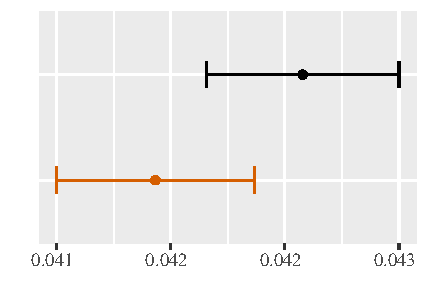
\includegraphics[height=.18\textheight, clip=true, trim=0cm 0cm 0cm .2cm]{draft_figures/plots_pooled/BIT.pdf} &
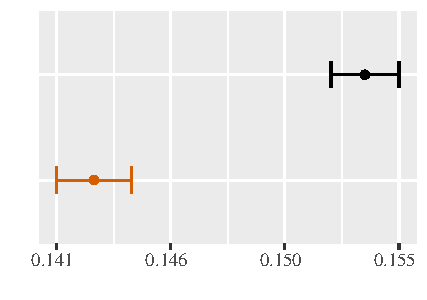
\includegraphics[height=.18\textheight, clip=true, trim=0cm 0cm 0cm .2cm]{draft_figures/plots_pooled/DefenseTreaty.pdf}   \\
Product of Dyad's GDP & Distance\\
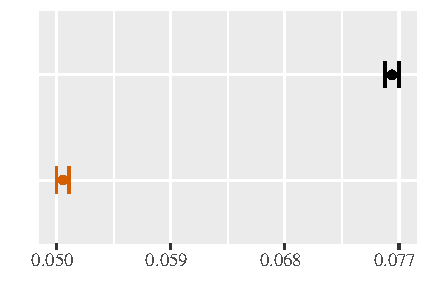
\includegraphics[height=.18\textheight, clip=true, trim=0cm 0cm 0cm .2cm]{draft_figures/plots_pooled/DyadGDPProduct.pdf} &
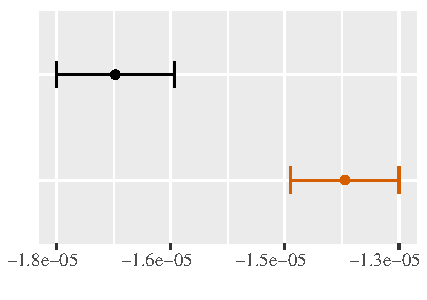
\includegraphics[height=.18\textheight, clip=true, trim=0cm 0cm 0cm .2cm]{draft_figures/plots_pooled/Distance.pdf}   \\
\pagebreak
Lagged FDI stock & Bilateral Trade Volume \\
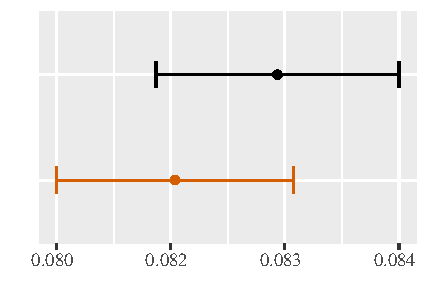
\includegraphics[height=.18\textheight, clip=true, trim=0cm 0cm 0cm .2cm]{draft_figures/plots_pooled/LaggedDV.pdf}    &
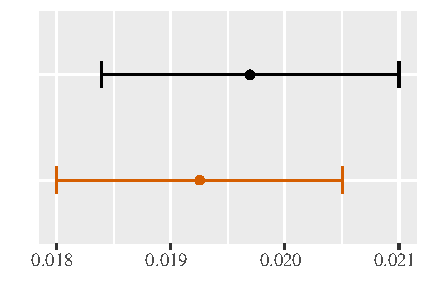
\includegraphics[height=.18\textheight, clip=true, trim=0cm 0cm 0cm .2cm]{draft_figures/plots_pooled/TradeVolume.pdf}   \\
GDP per capita, in-degree & GDP per capita, out-degree\\
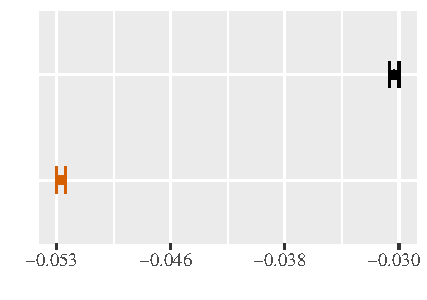
\includegraphics[height=.18\textheight, clip=true, trim=0cm 0cm 0cm .2cm]{draft_figures/plots_pooled/GDPpc_in.pdf} &
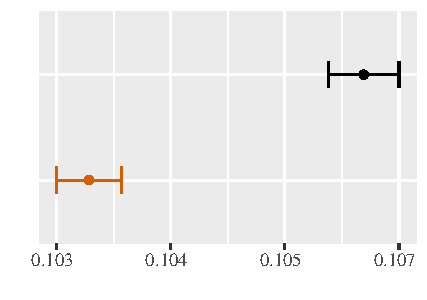
\includegraphics[height=.18\textheight, clip=true, trim=0cm 0cm 0cm .2cm]{draft_figures/plots_pooled/GDPpc_out.pdf}   \\
Polity, in-degree & Polity, out-degree\\
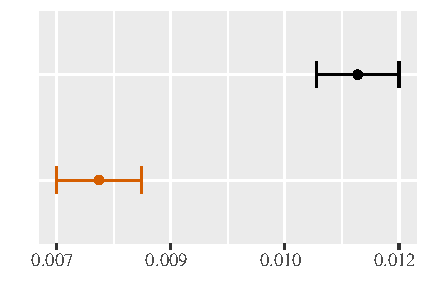
\includegraphics[height=.18\textheight, clip=true, trim=0cm 0cm 0cm .2cm]{draft_figures/plots_pooled/Polity_in.pdf} &
\includegraphics[height=.18\textheight, clip=true, trim=0cm 0cm 0cm .2cm]{draft_figures/plots_pooled/Polity_out.pdf}   \\
Trade Openness, in-degree & Trade Openness, out-degree\\
\includegraphics[height=.18\textheight, clip=true, trim=0cm 0cm 0cm .2cm]{draft_figures/plots_pooled/Trade_in.pdf} &
\includegraphics[height=.18\textheight, clip=true, trim=0cm 0cm 0cm .2cm]{draft_figures/plots_pooled/Trade_out.pdf}   \\

\caption{\label{fig:effectPlots2} Estimates of terms in time-pooled ERGMs. Bars span 95\% confidence intervals. Black coefficient representations are from models excluding dependence terms (i.e., transitivity and reciprocity).}

\end{longtable}


\section{Subset by Missingness Results}\label{qlevelresults}

To subset the data based on the level of missingness, we approximate total level of missingness ({\emph{q}) in the adjacency matrices by using the proportion of missing values for each node (\emph{p}). When \emph{p} = 0.72, \emph{q} $\approx$ 0.25 and  \emph{n} = 28. When \emph{p} = 0.86,  \emph{q} $\approx$ 0.50 and  \emph{n} = 70.

\subsection{q $\approx$  0.50}

\begin{figure}[!h]
\centering
\begin{tabular}{c@{\hskip 0cm}c}
Reciprocity & Transitivity \\
\includegraphics[height=.2\textheight, clip=true, trim=0cm 0cm 0cm .2cm]{draft_figures/rl_plots50/Mutuality.pdf}    &
\includegraphics[height=.2\textheight, clip=true, trim=0cm 0cm 0cm .2cm]{draft_figures/rl_plots50/Transitivity.pdf}
\end{tabular}
\caption{\label{fig:exog_2} Estimates of Dependence terms. Bars span 95\% confidence intervals. }
\end{figure}





\subsection{q $\approx$  0.25}

\begin{figure}[!h]
\centering
\begin{tabular}{c@{\hskip 0cm}c}
Reciprocity & Transitivity \\
\includegraphics[height=.2\textheight, clip=true, trim=0cm 0cm 0cm .2cm]{draft_figures/rl_plots25/Mutuality.pdf}    &
\includegraphics[height=.2\textheight, clip=true, trim=0cm 0cm 0cm .2cm]{draft_figures/rl_plots25/Transitivity.pdf}
\end{tabular}
\caption{\label{fig:q25netterms} Estimates of Dependence terms. Bars span 95\% confidence intervals. }
\end{figure}








\section{Multiple Imputations with Amelia Results}\label{ameliaresults}

We use the \R{} Amelia  package to create 10 datasets of imputed FDI stock values for the full dataset and when \emph{q} $\approx$ 0.05 \citep{honaker2011amelia}.

\subsection{Full}

\begin{figure}[!h]
\centering
\begin{tabular}{c@{\hskip 0cm}c}
Reciprocity & Transitivity \\
\includegraphics[height=.2\textheight, clip=true, trim=0cm 0cm 0cm .2cm]{draft_figures/rl_amelia_full/Mutuality.pdf}    &
\includegraphics[height=.2\textheight, clip=true, trim=0cm 0cm 0cm .2cm]{draft_figures/rl_amelia_full/Transitivity.pdf}
\end{tabular}
\caption{\label{fig:full_amelia_netterms} Estimates of Dependence terms Bars span 95\% confidence intervals. }
\end{figure}








\subsection{q $\approx$ 0.50}

\begin{figure}[!h]
\centering
\begin{tabular}{c@{\hskip 0cm}c}
Reciprocity & Transitivity \\
\includegraphics[height=.2\textheight, clip=true, trim=0cm 0cm 0cm .2cm]{draft_figures/rl_amelia_q50/Mutuality.pdf}    &
\includegraphics[height=.2\textheight, clip=true, trim=0cm 0cm 0cm .2cm]{draft_figures/rl_amelia_q50/Transitivity.pdf}
\end{tabular}
\caption{\label{fig:q50_amelia_netterms} Estimates of Dependence terms in time-pooled ERGMs. Bars span 95\% confidence intervals. }
\end{figure}








\end{document}



Table \ref{tab:describe_binary} provides means for the dichotomous dyadic variables used in our models....

% Table created by stargazer v.5.2 by Marek Hlavac, Harvard University. E-mail: hlavac at fas.harvard.edu
% Date and time: Mon, Feb 20, 2017 - 22:08:59
\begin{table}[htp] \centering
  \caption{}
  \label{}
\begin{tabular}{@{\extracolsep{5pt}}lcccc}
\\[-1.8ex]\hline
\hline \\[-1.8ex]
Statistic &  \multicolumn{1}{c}{Mean} & \multicolumn{1}{c}{St. Dev.} & \multicolumn{1}{c}{Min} & \multicolumn{1}{c}{Max} \\
\hline \\[-1.8ex]
Contiguity &  0.024 & 0.152 & 0 & 1 \\
Common Official Language &  0.112 & 0.315 & 0 & 1 \\
Common Language and Ethnicity &  0.115 & 0.318 & 0 & 1 \\
Former Colonial Relationship &  0.015 & 0.121 & 0 & 1 \\
Common Colonizer &  0.062 & 0.241 & 0 & 1 \\
Defense Treaty &  0.075 & 0.264 & 0 & 1 \\
Non-aggression Treaty &  0.064 & 0.245 & 0 & 1 \\
Neutrality Treaty &  0.004 & 0.063 & 0 & 1 \\
Entente Treaty &  0.066 & 0.248 & 0 & 1 \\
\hline \\[-1.8ex]
\end{tabular}
\caption{\label{tab:describe_binary} Descriptive statistics for dichotomous dyadic covariates. Number of observations across all years is 189,000.}
\end{table}


\includegraphics[scale=.8]{draft_figures/reciprocity.png}\\
\includegraphics[scale=.8]{draft_figures/transitivity.png}\\
\includegraphics[scale=.8]{draft_figures/assortativity.png}\\
